\subsection{Introducción.}
\begin{frame}
  \frametitle{Motivación.}
  Queremos obtener el polígono de visibilidad $V(q)$ dado un punto $q$ y un polígono
  simple $P$.\newline

  \textbf{Obs.} Si
  \[V(q) = P,\]
  entonces $P$ es un polígono estrellado.\newline

  Asumimos que el polígono a trabajar no tiene un número de revoluciones mayor a $1$.
\end{frame}

\subsection{Ejecución.}
\begin{frame}
  \centering 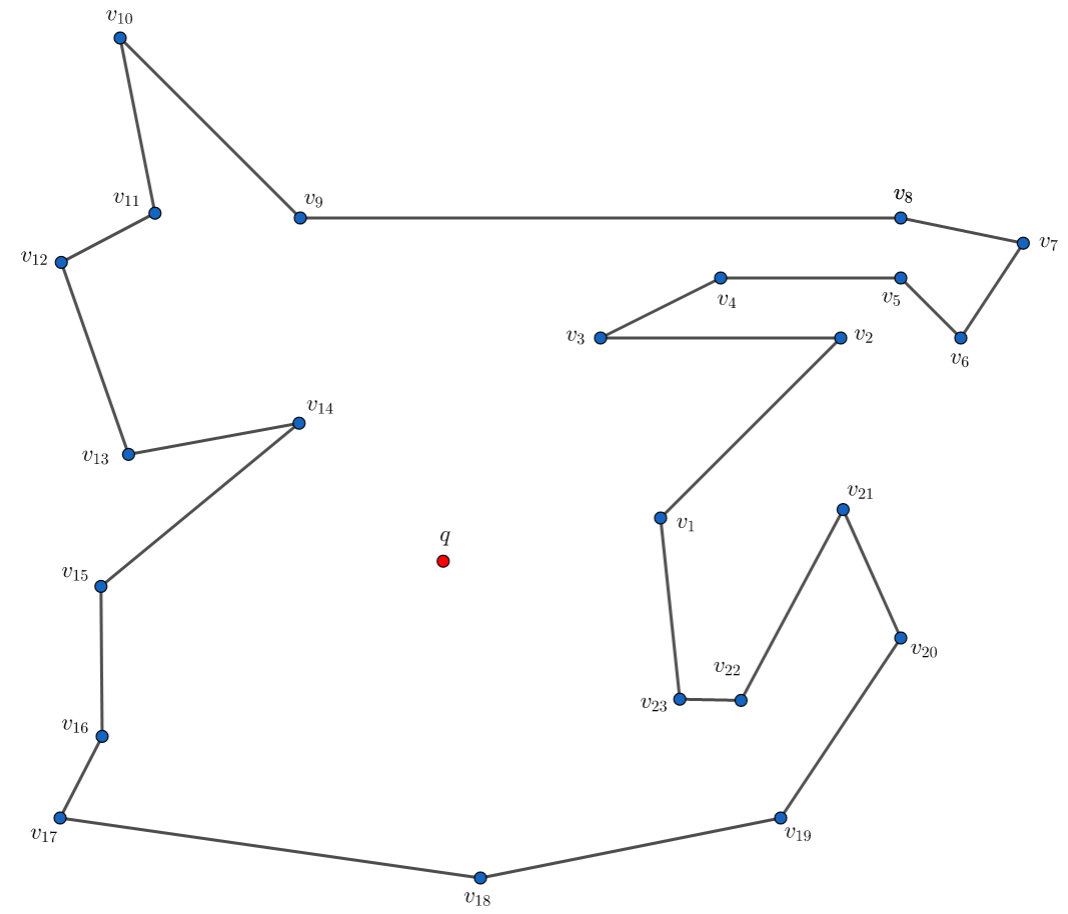
\includegraphics[width=0.70 \paperwidth]{images/Ejecucion/e01.png}
\end{frame}

\begin{frame}
  \centering 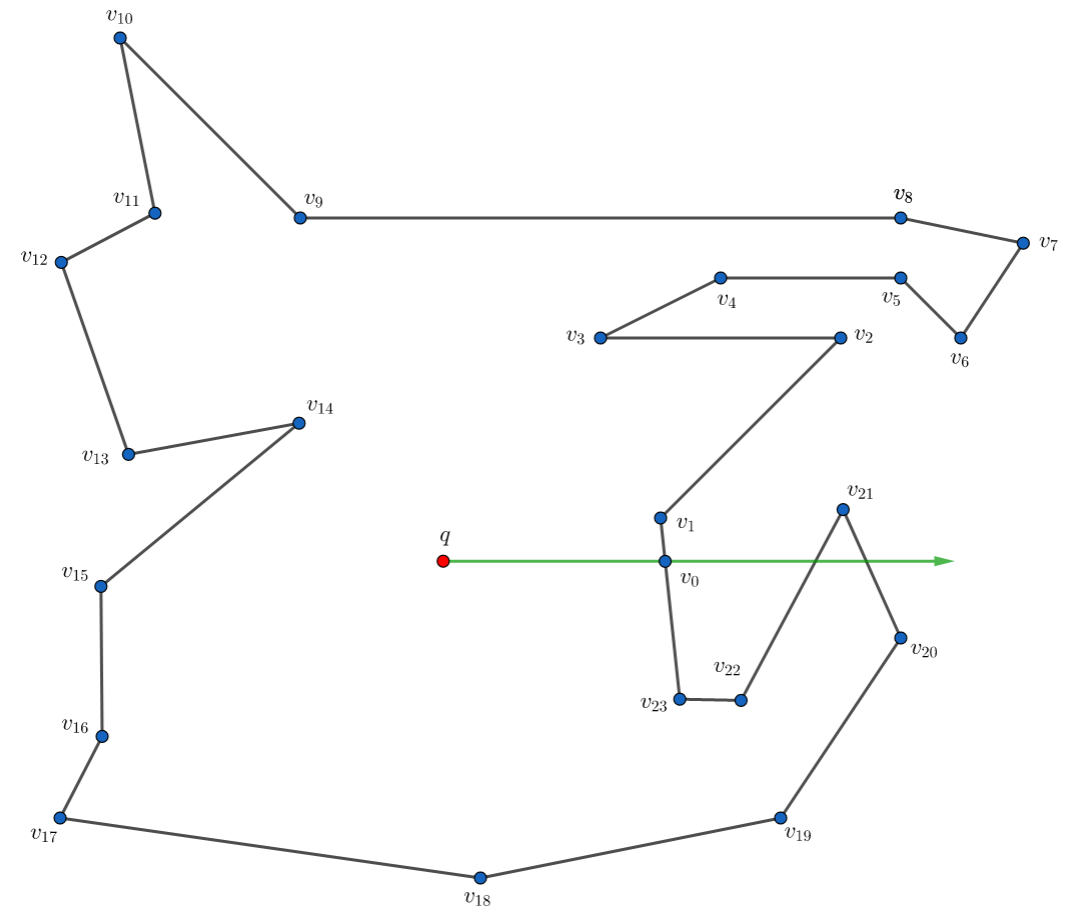
\includegraphics[width=0.70 \paperwidth]{images/Ejecucion/e02.png}
\end{frame}

\begin{frame}
  \centering 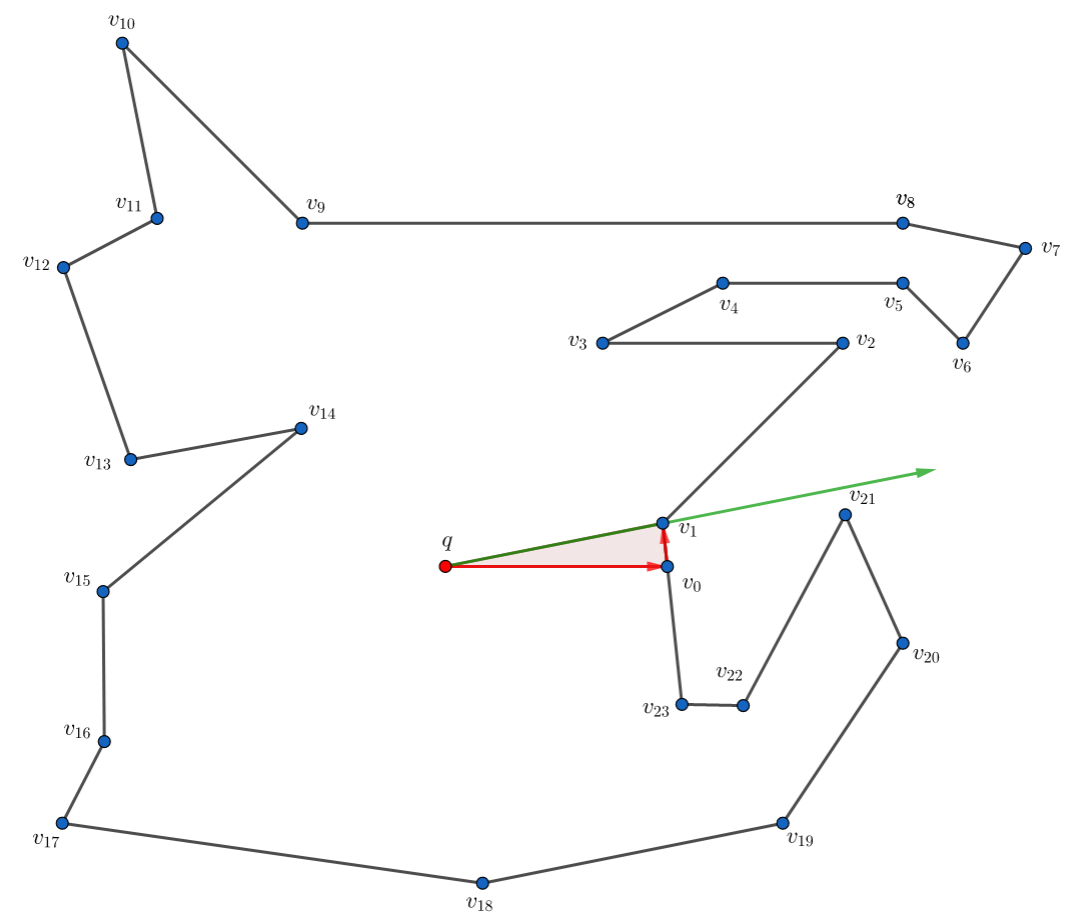
\includegraphics[width=0.70 \paperwidth]{images/Ejecucion/e03.png}
\end{frame}

\begin{frame}
  \centering 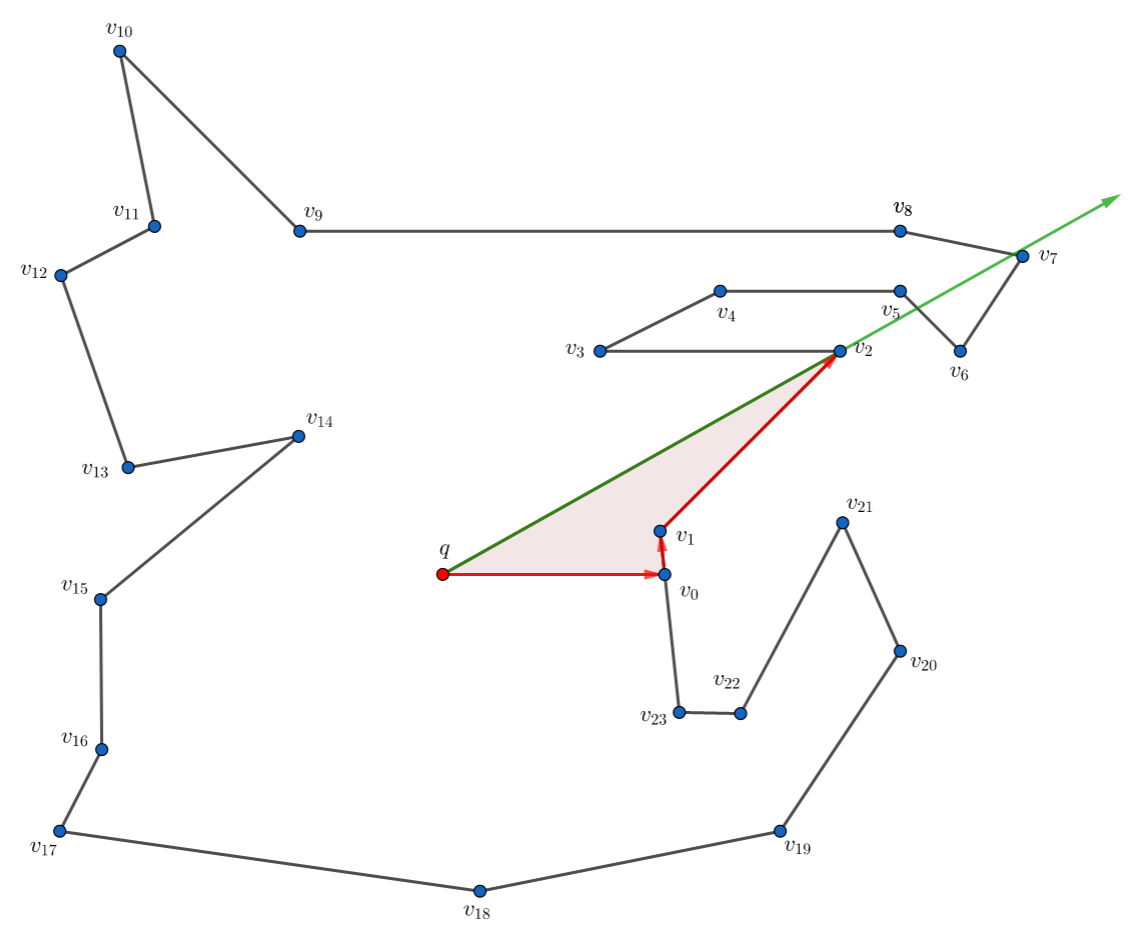
\includegraphics[width=0.70 \paperwidth]{images/Ejecucion/e04.png}
\end{frame}

\begin{frame}
  \centering 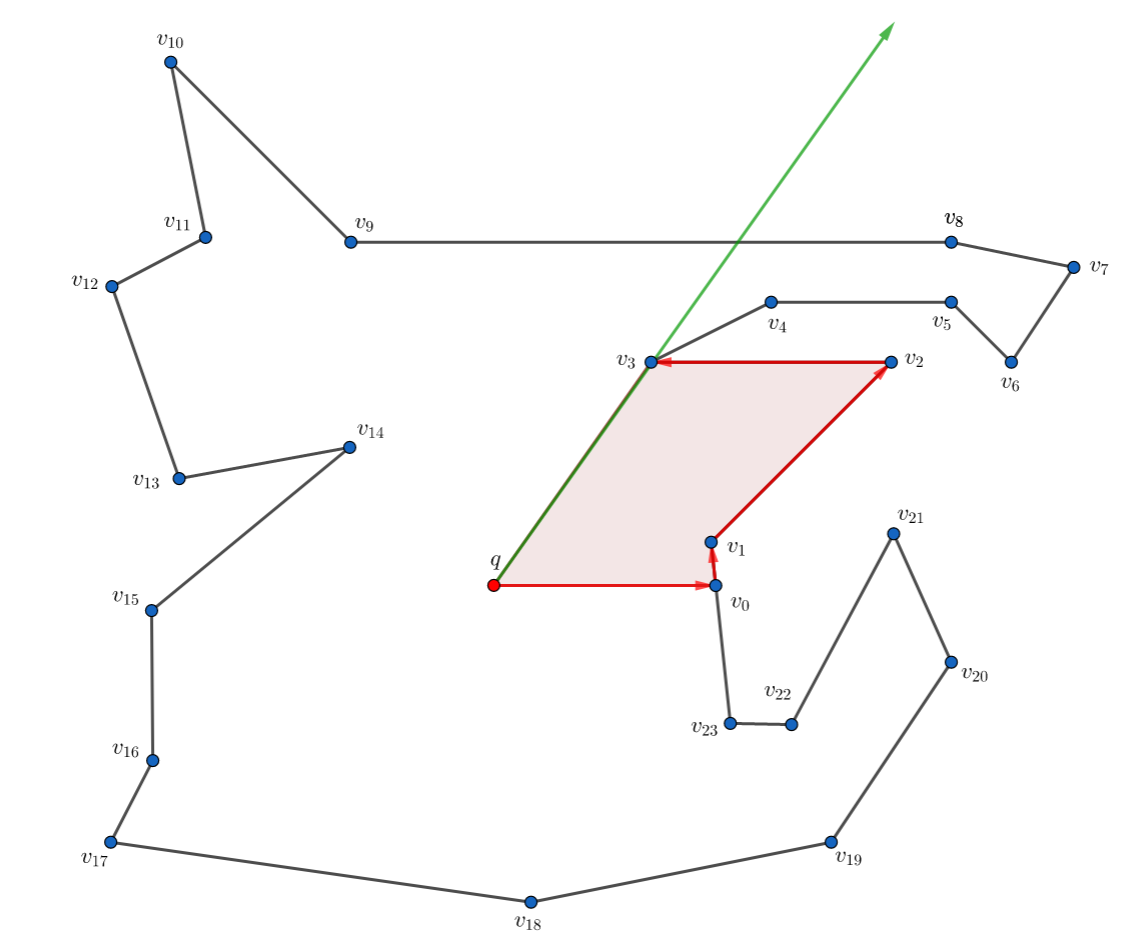
\includegraphics[width=0.70 \paperwidth]{images/Ejecucion/e05.png}
\end{frame}

\begin{frame}
  \centering 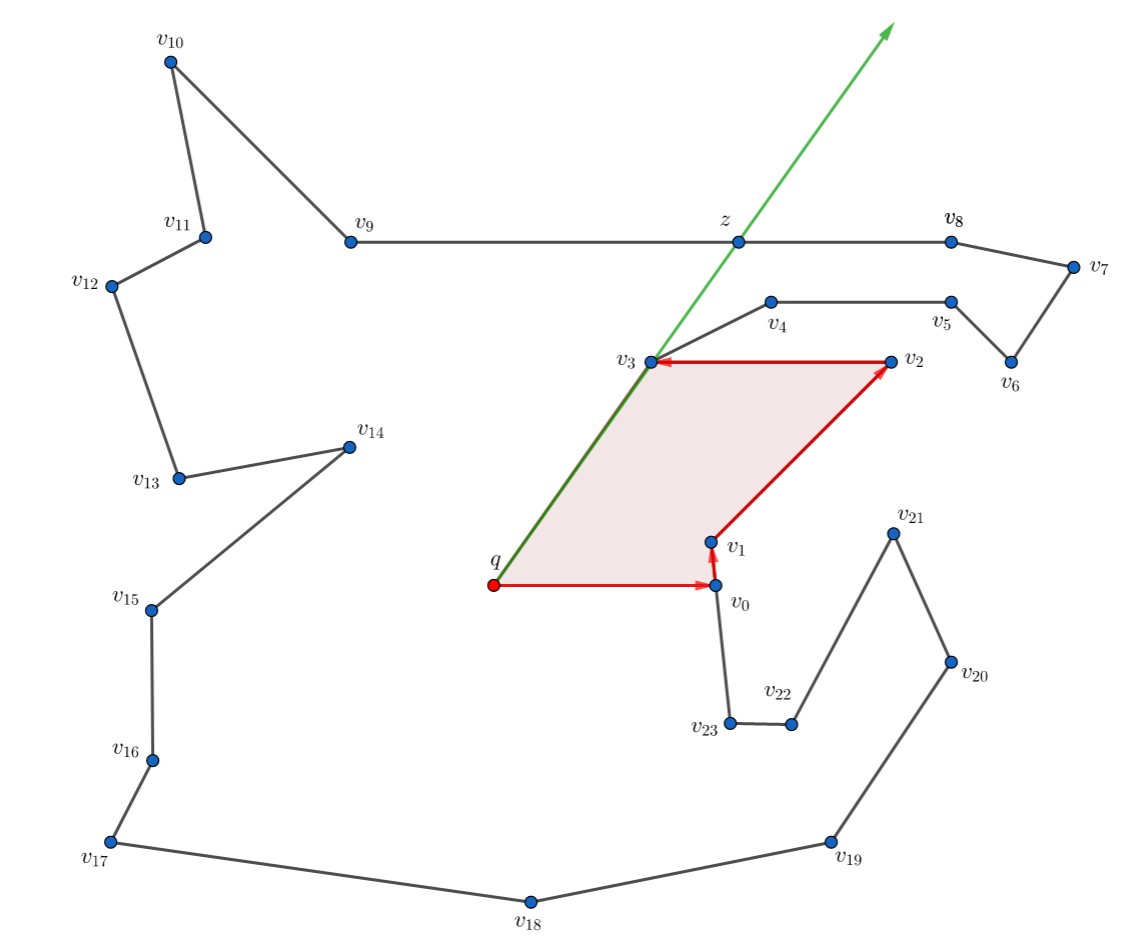
\includegraphics[width=0.70 \paperwidth]{images/Ejecucion/e06.png}
\end{frame}

\begin{frame}
  \centering 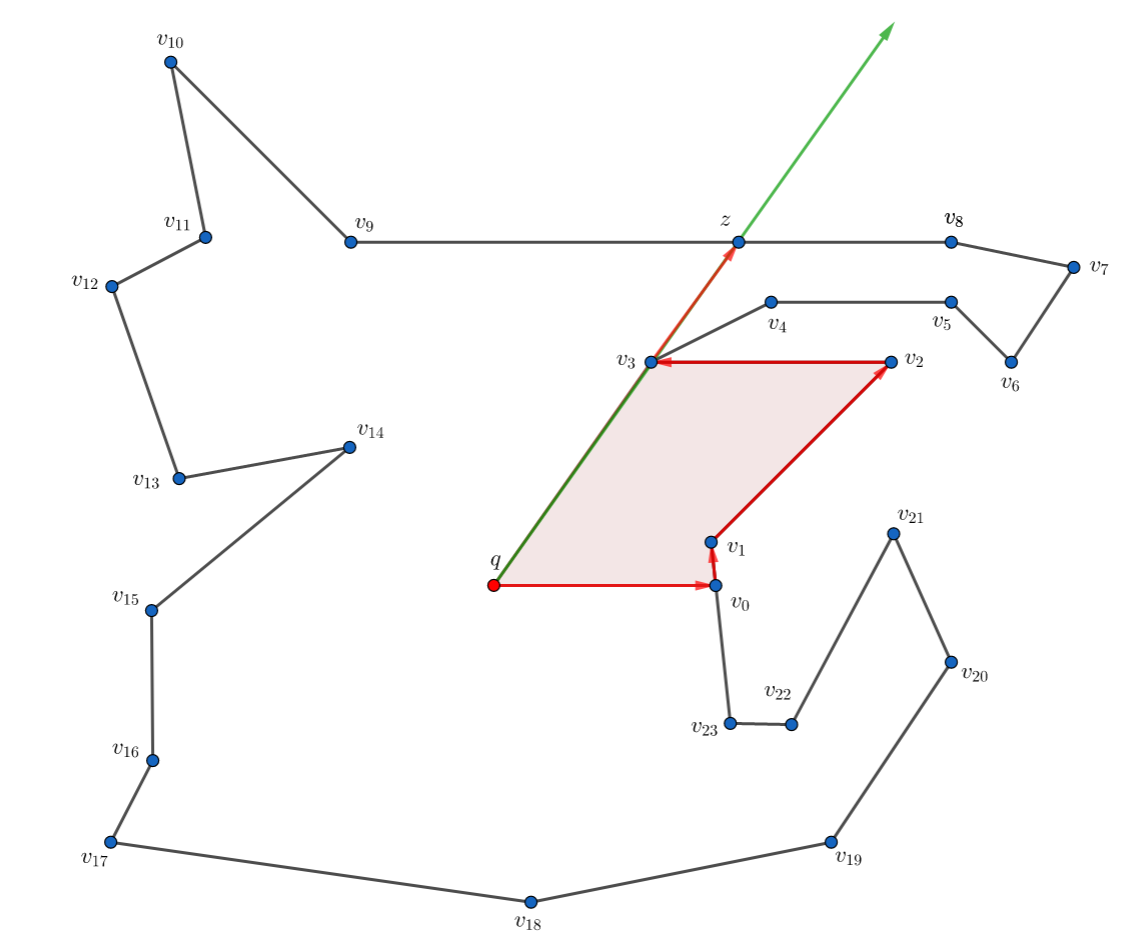
\includegraphics[width=0.70 \paperwidth]{images/Ejecucion/e07.png}
\end{frame}

\begin{frame}
  \centering 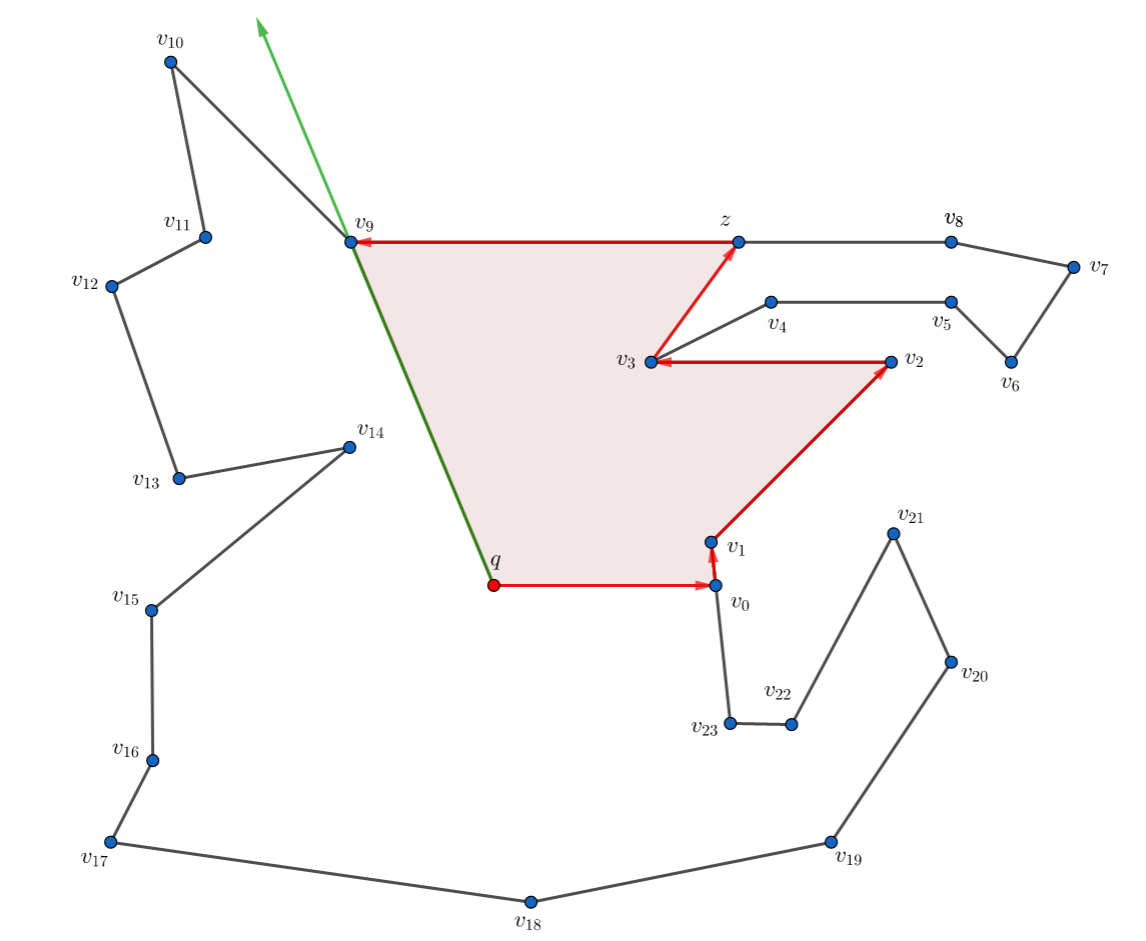
\includegraphics[width=0.70 \paperwidth]{images/Ejecucion/e08.png}
\end{frame}

\begin{frame}
  \centering 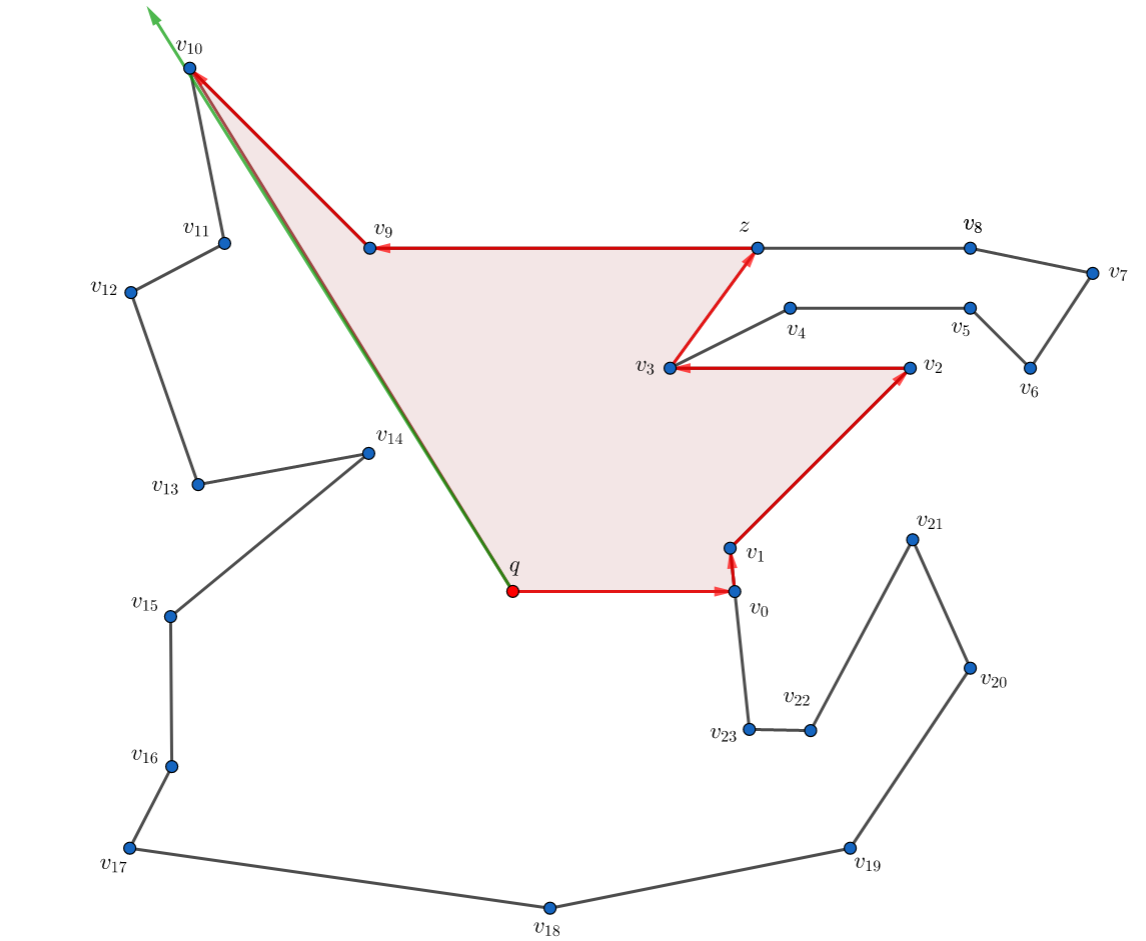
\includegraphics[width=0.70 \paperwidth]{images/Ejecucion/e09.png}
\end{frame}

\begin{frame}
  \centering 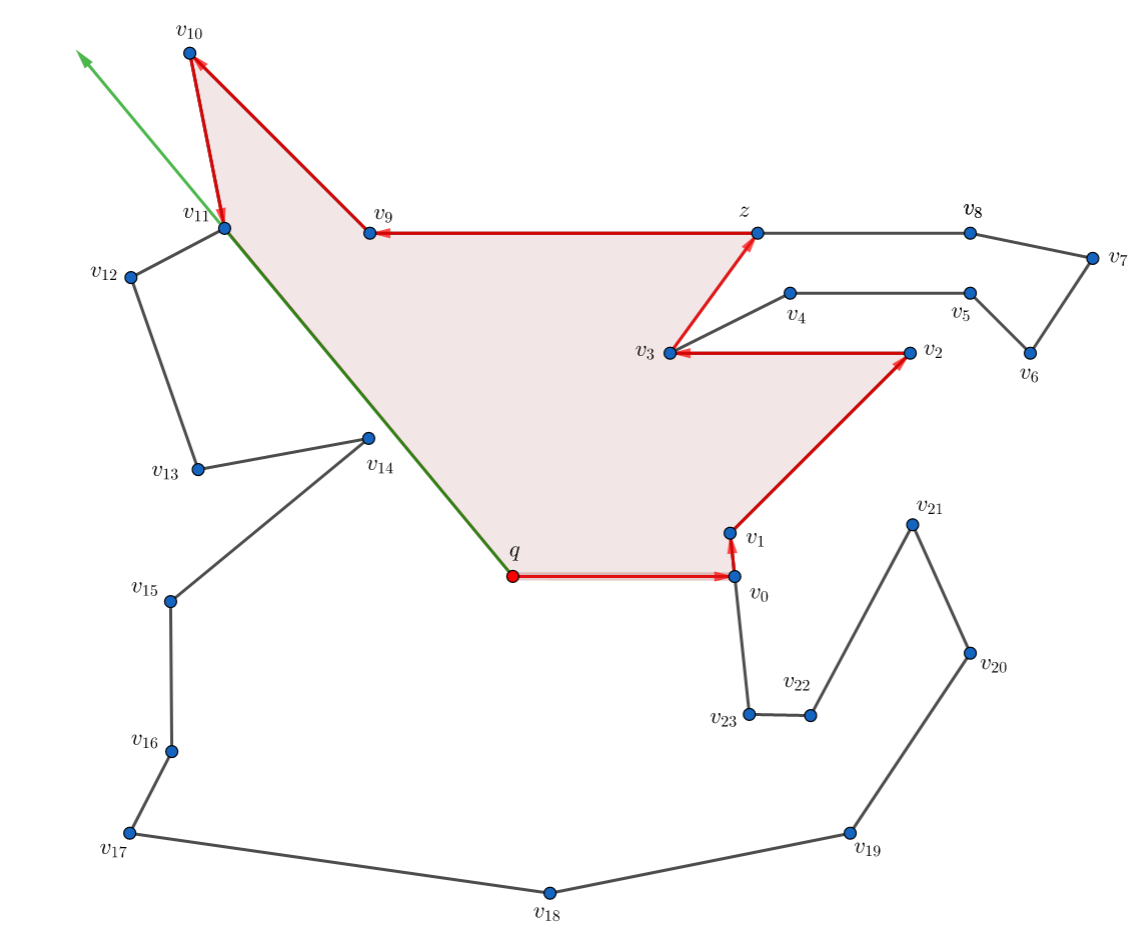
\includegraphics[width=0.70 \paperwidth]{images/Ejecucion/e10.png}
\end{frame}

\begin{frame}
  \centering 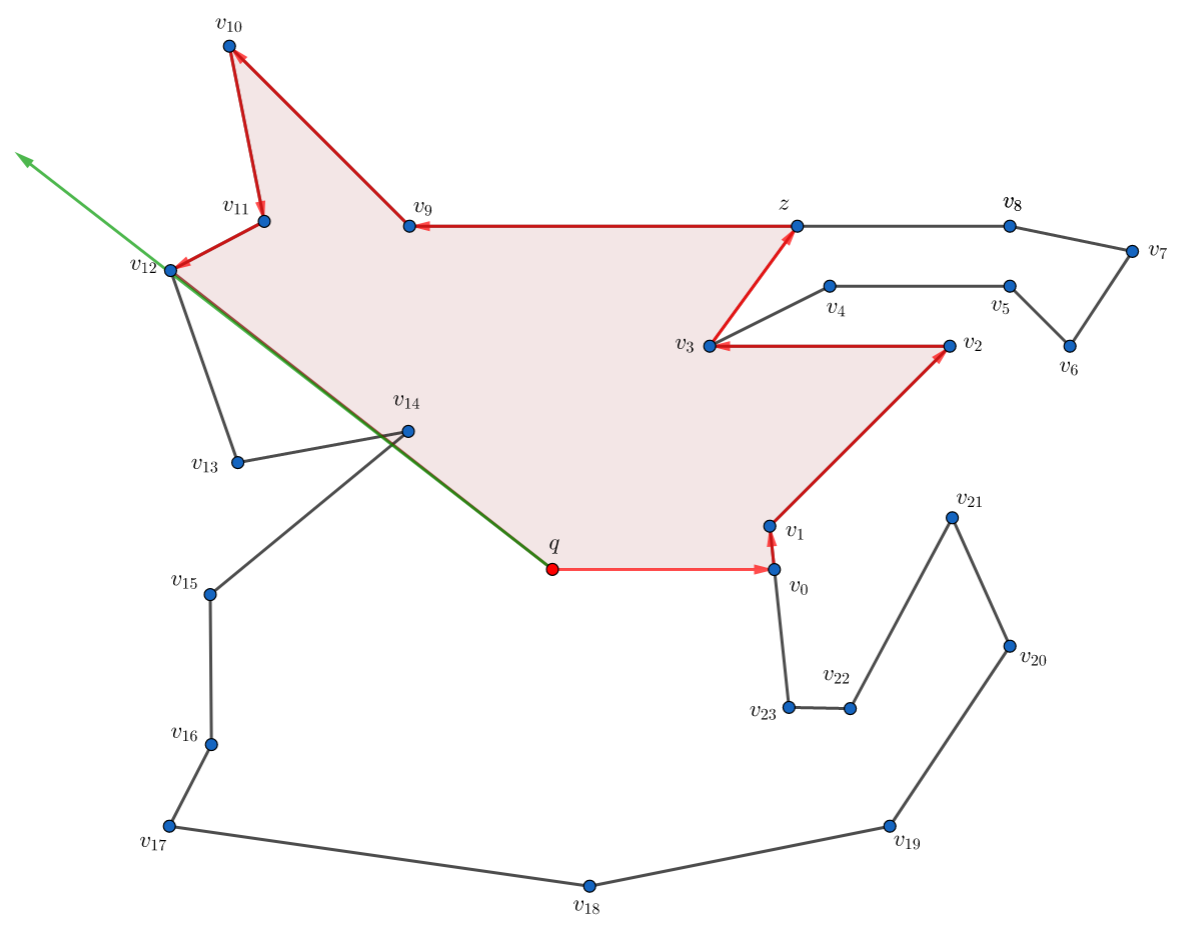
\includegraphics[width=0.70 \paperwidth]{images/Ejecucion/e11.png}
\end{frame}

\begin{frame}
  \centering 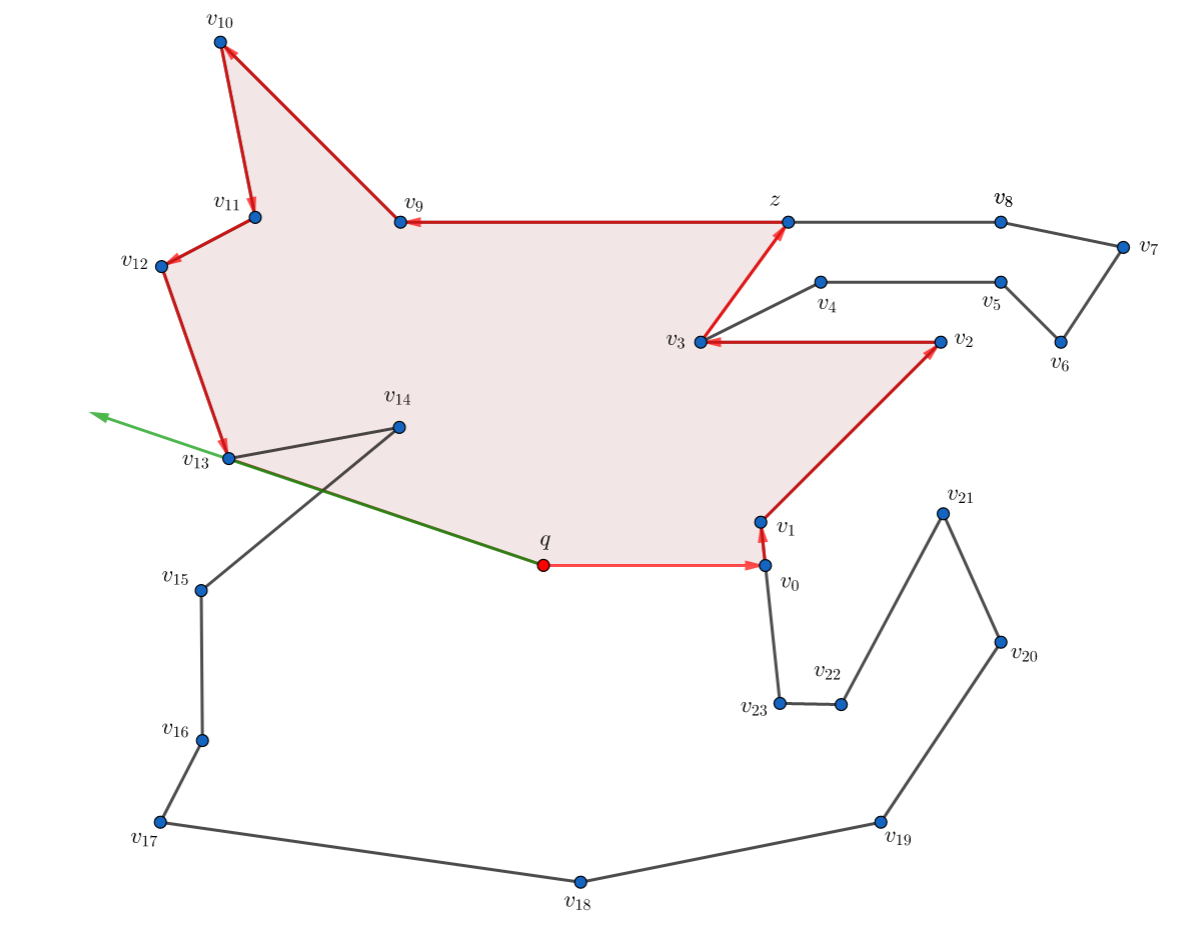
\includegraphics[width=0.70 \paperwidth]{images/Ejecucion/e12.png}
\end{frame}

\begin{frame}
  \centering 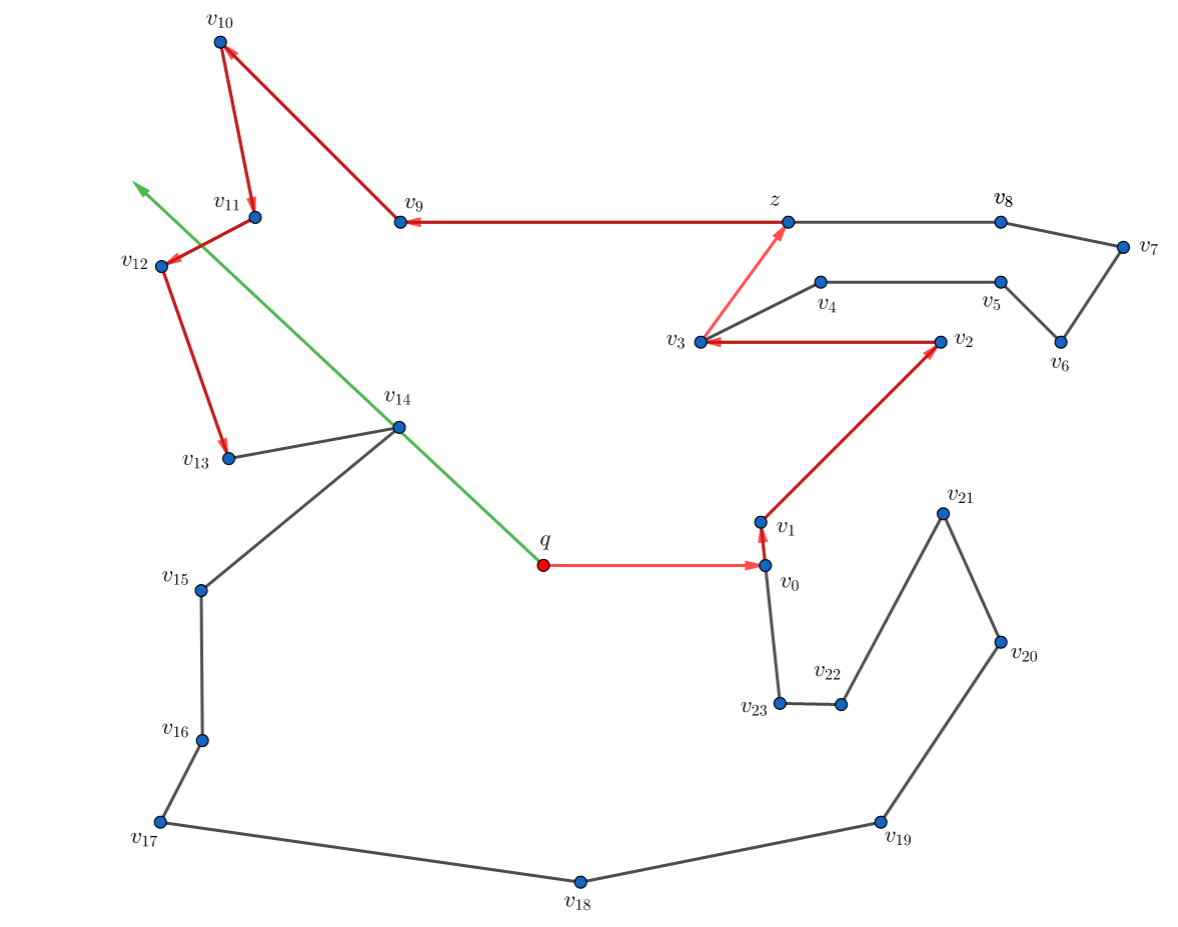
\includegraphics[width=0.70 \paperwidth]{images/Ejecucion/e13.png}
\end{frame}

\begin{frame}
  \centering 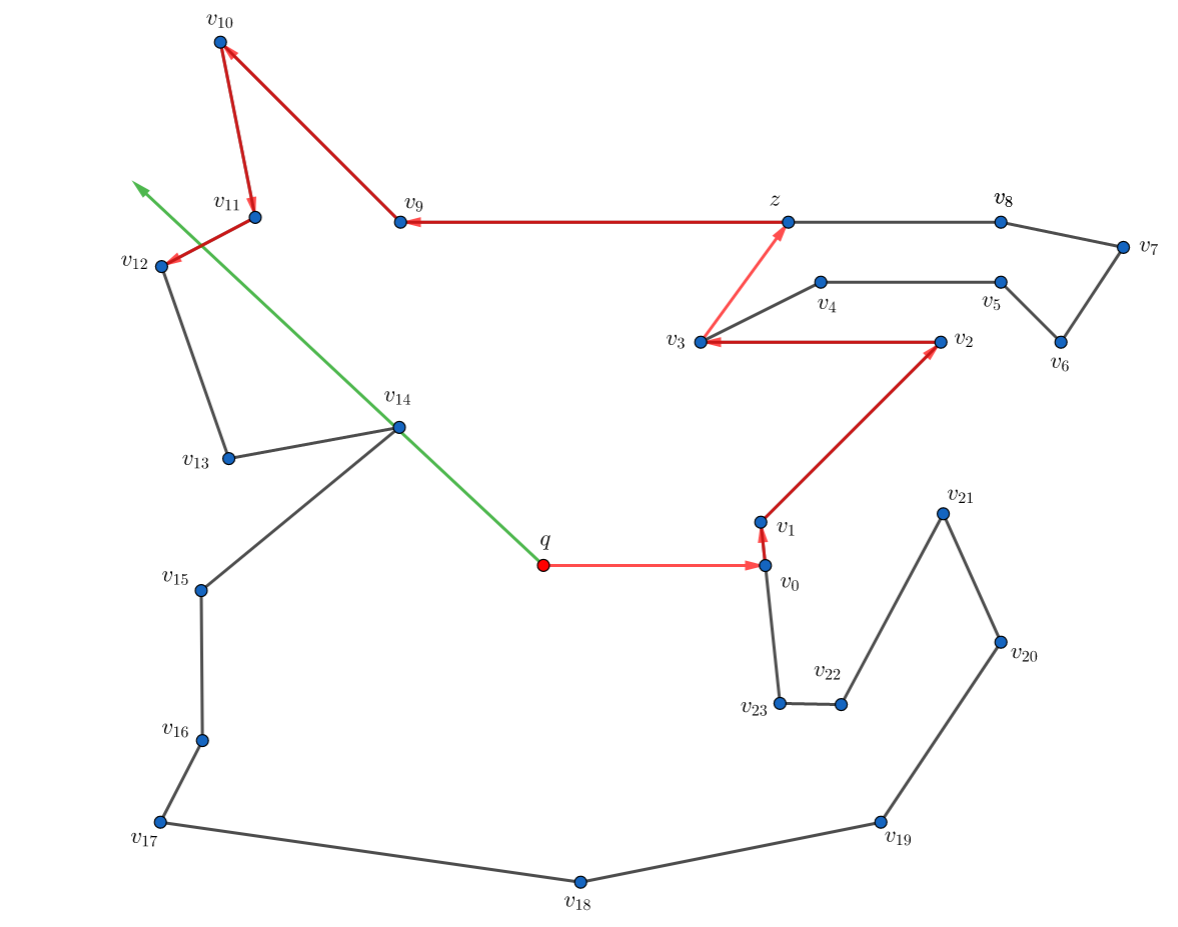
\includegraphics[width=0.70 \paperwidth]{images/Ejecucion/e14.png}
\end{frame}

\begin{frame}
  \centering 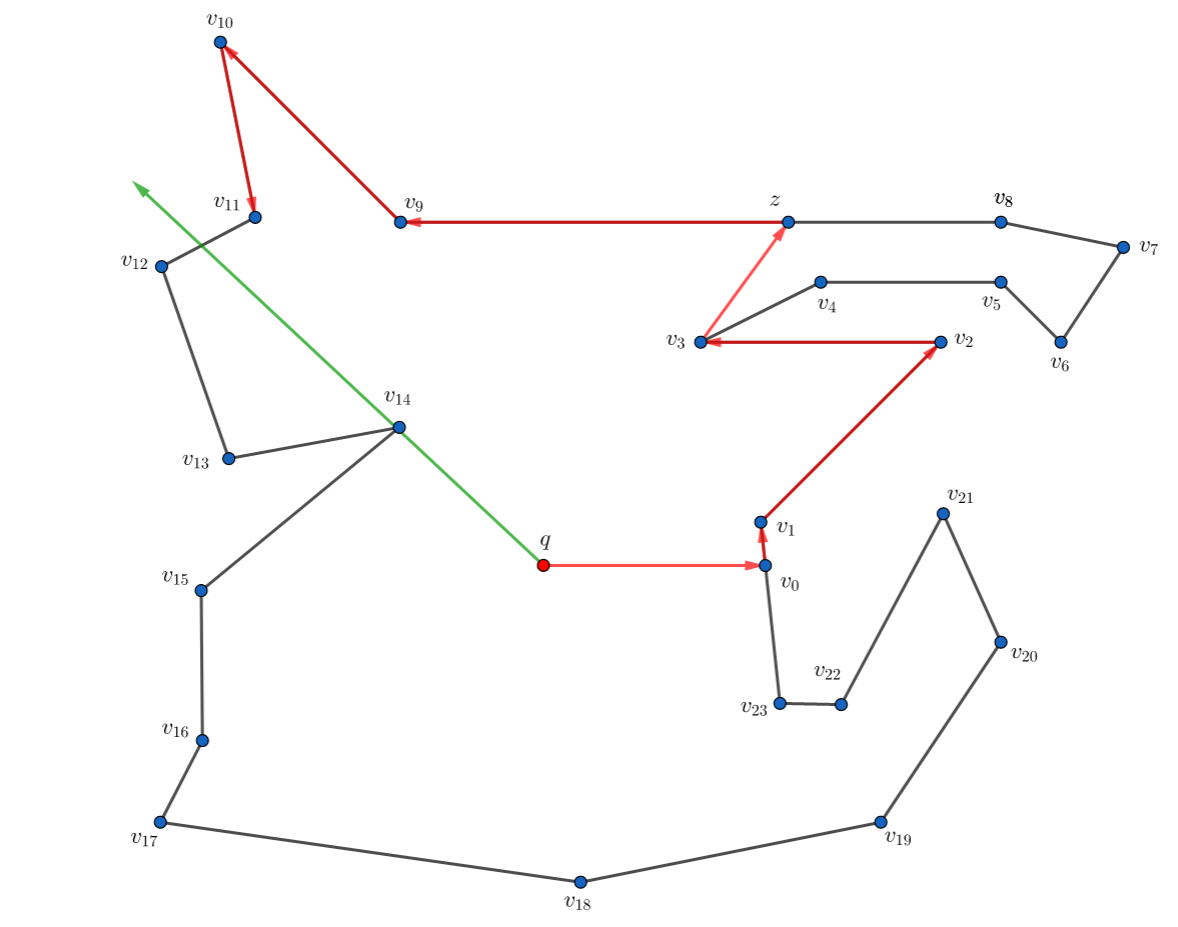
\includegraphics[width=0.70 \paperwidth]{images/Ejecucion/e15.png}
\end{frame}

\begin{frame}
  \centering 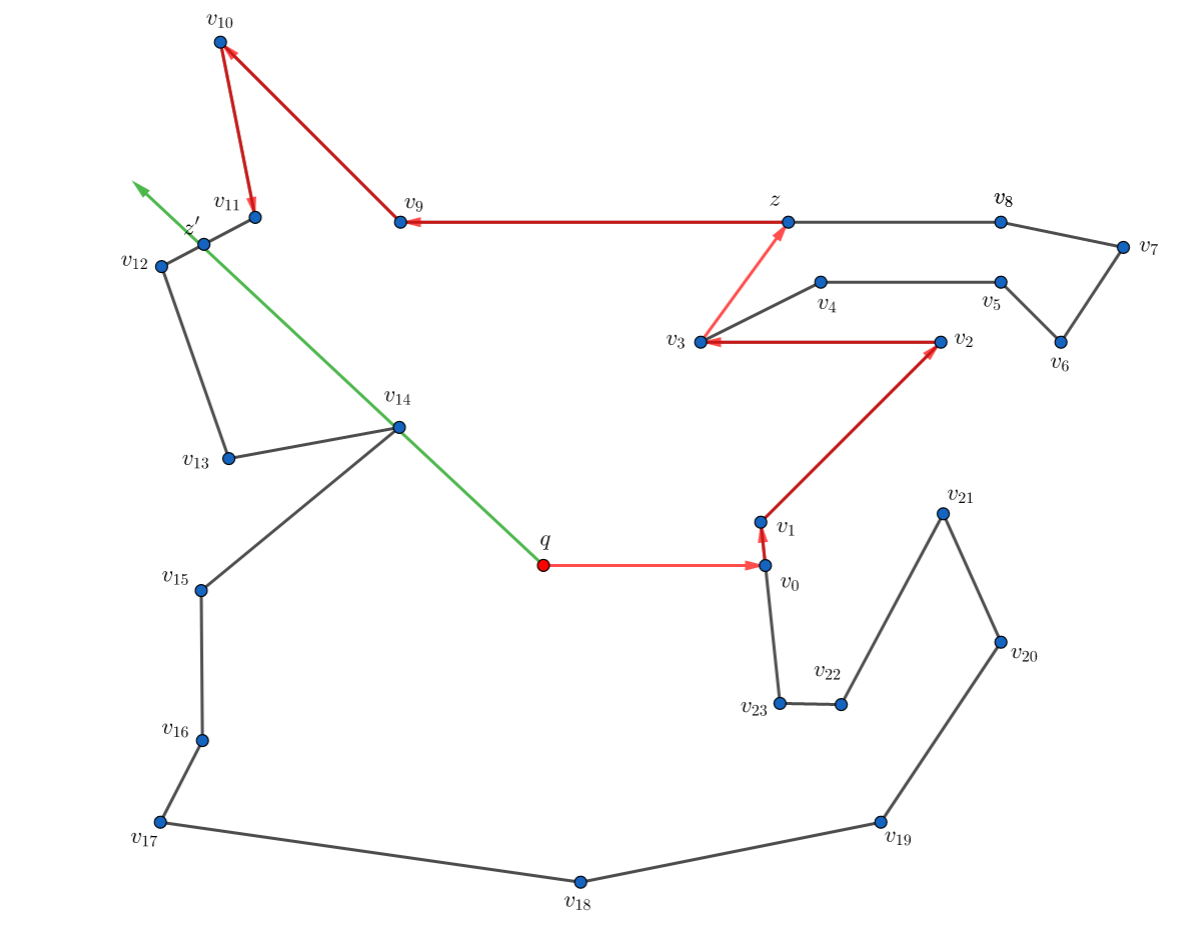
\includegraphics[width=0.70 \paperwidth]{images/Ejecucion/e16.png}
\end{frame}

\begin{frame}
  \centering 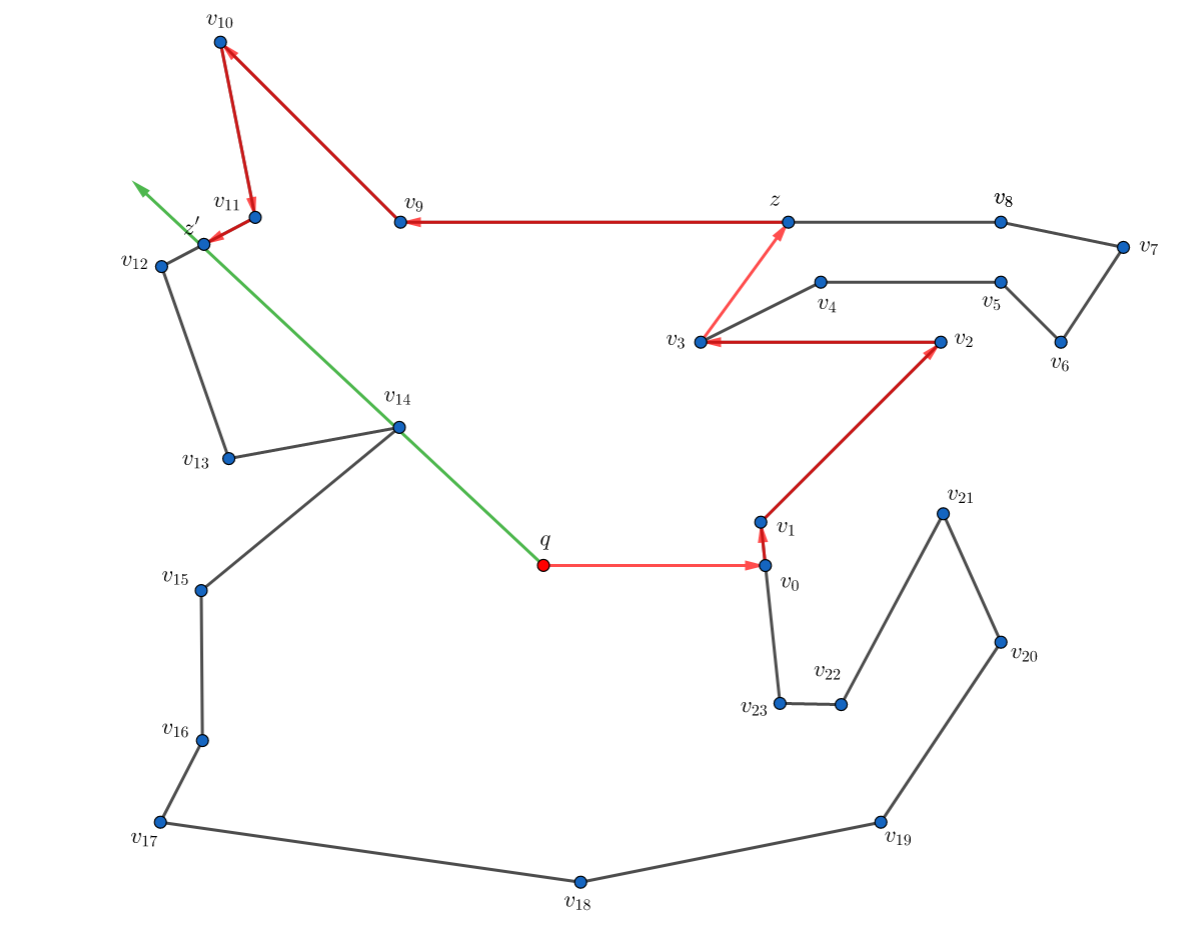
\includegraphics[width=0.70 \paperwidth]{images/Ejecucion/e17.png}
\end{frame}

\begin{frame}
  \centering 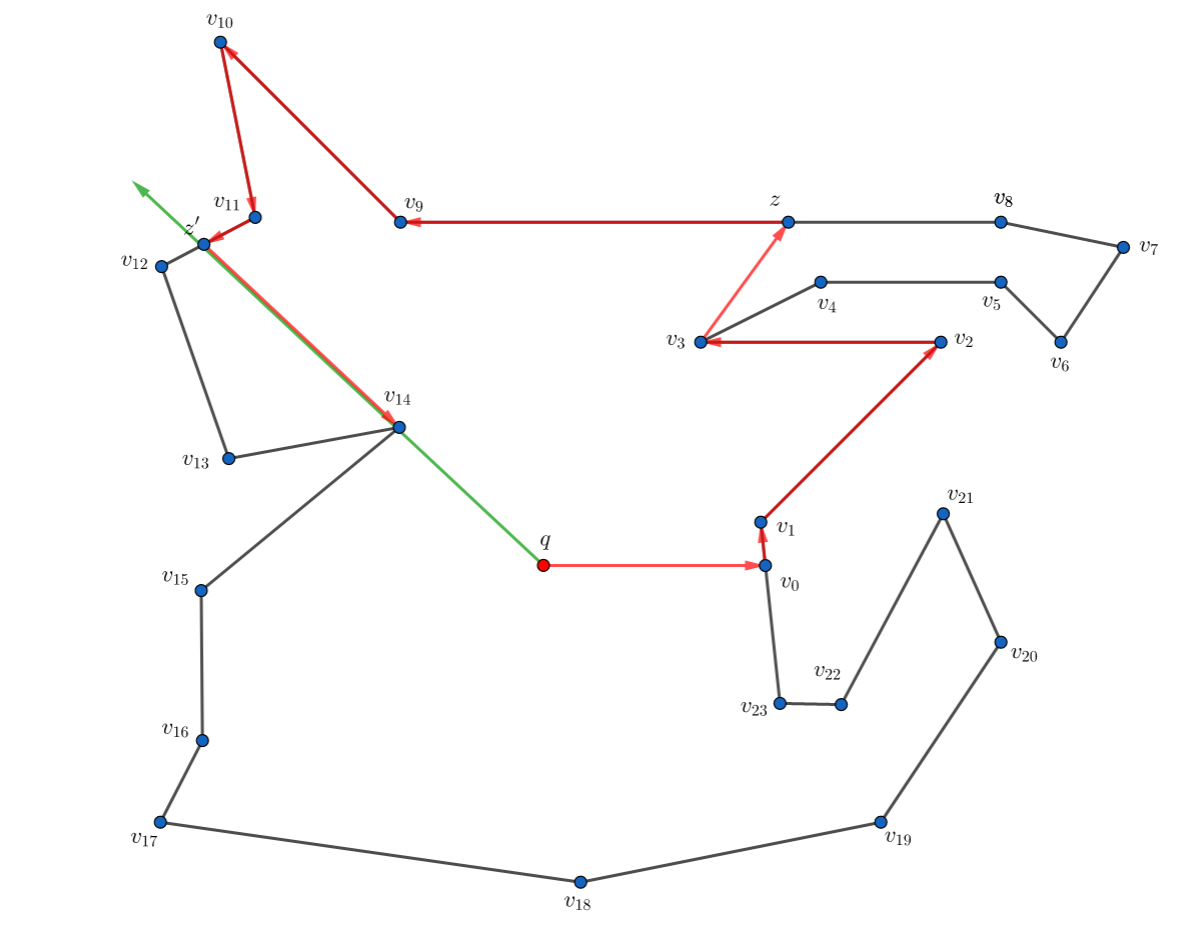
\includegraphics[width=0.70 \paperwidth]{images/Ejecucion/e18.png}
\end{frame}

\begin{frame}
  \centering 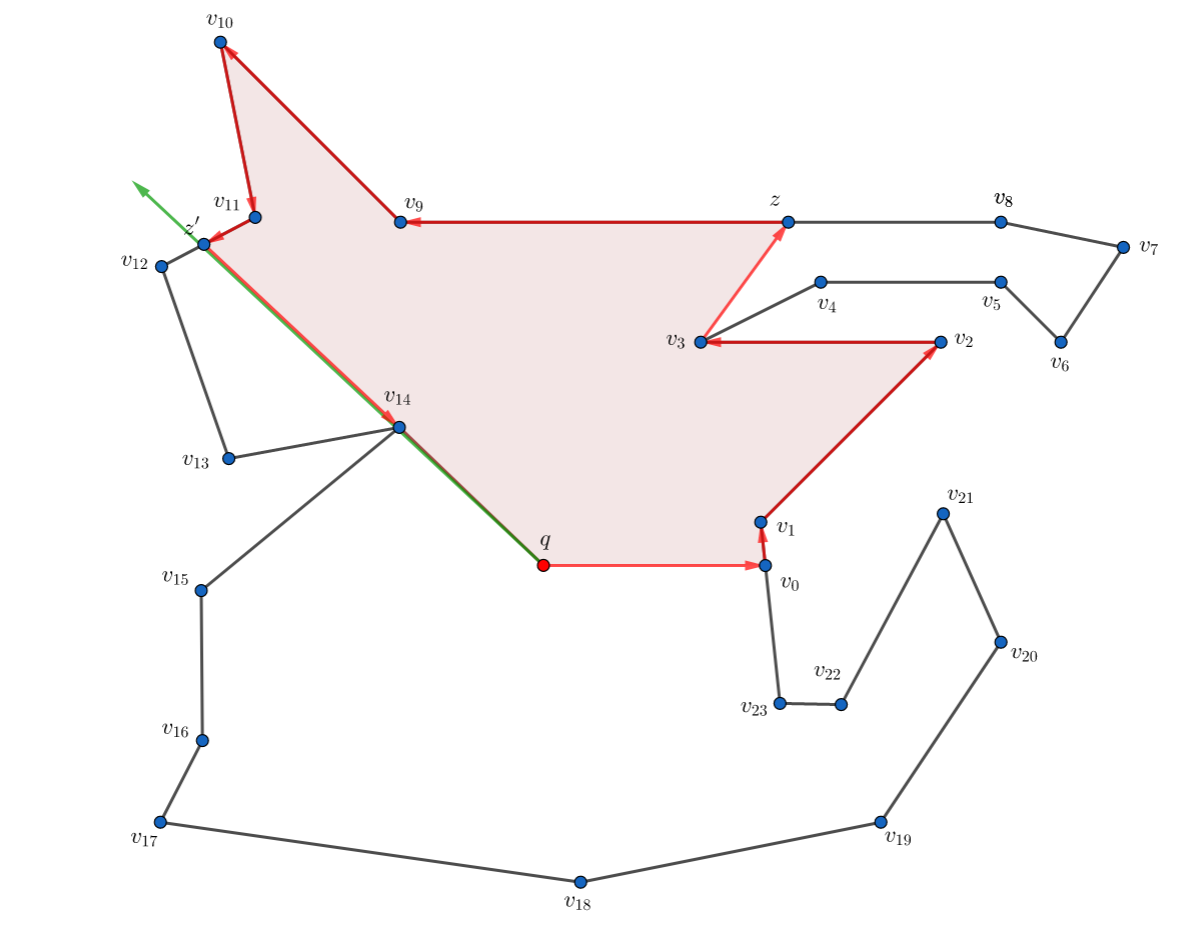
\includegraphics[width=0.70 \paperwidth]{images/Ejecucion/e19.png}
\end{frame}

\begin{frame}
  \centering 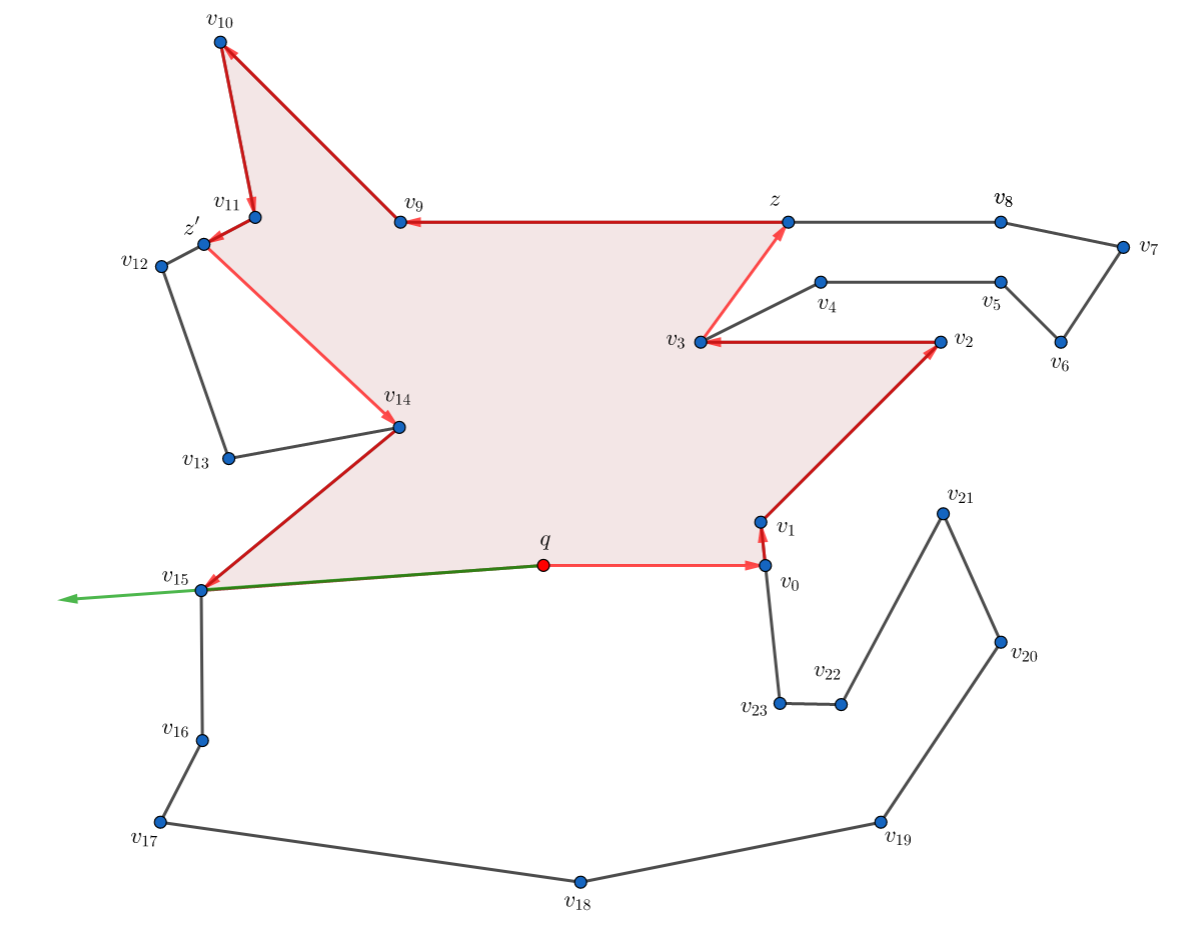
\includegraphics[width=0.70 \paperwidth]{images/Ejecucion/e20.png}
\end{frame}

\begin{frame}
  \centering 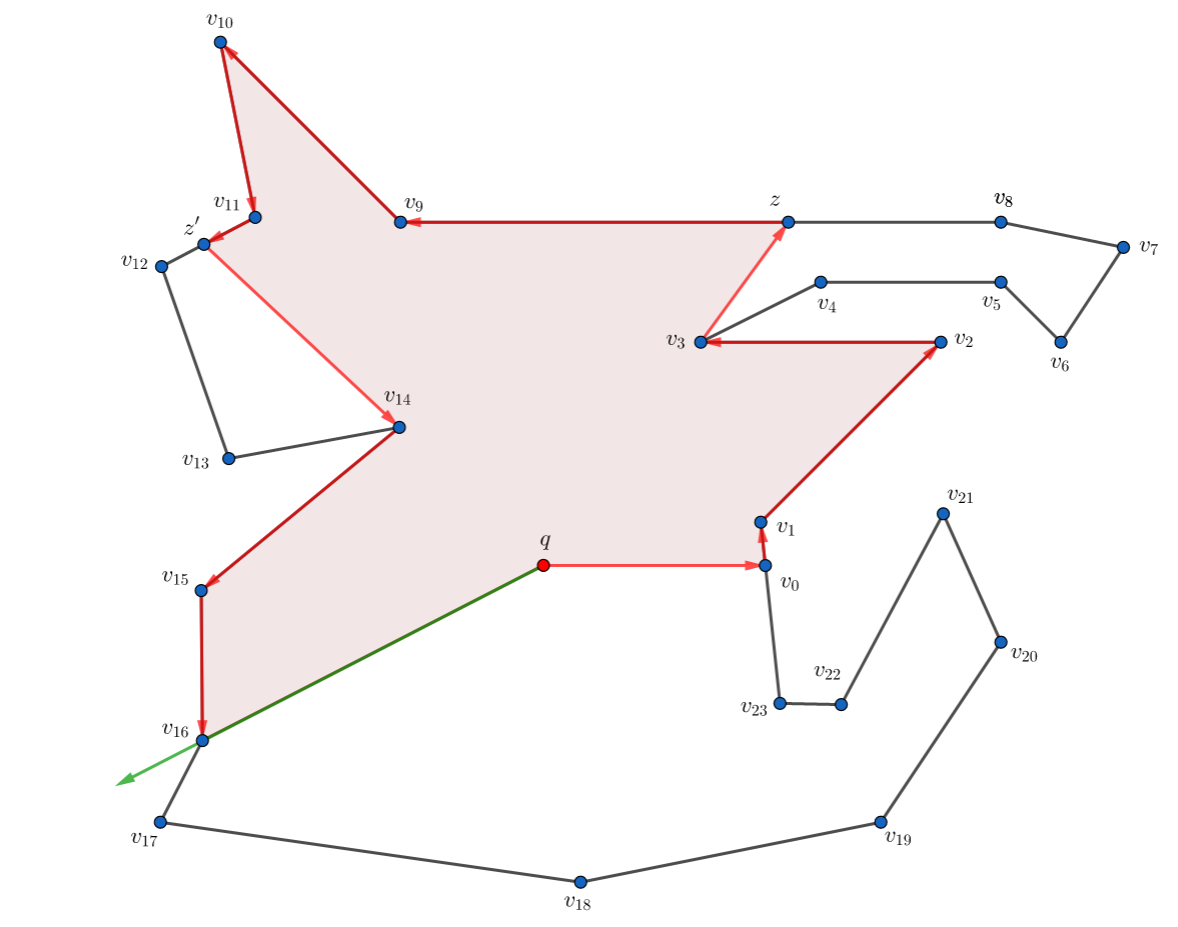
\includegraphics[width=0.70 \paperwidth]{images/Ejecucion/e21.png}
\end{frame}

\begin{frame}
  \centering 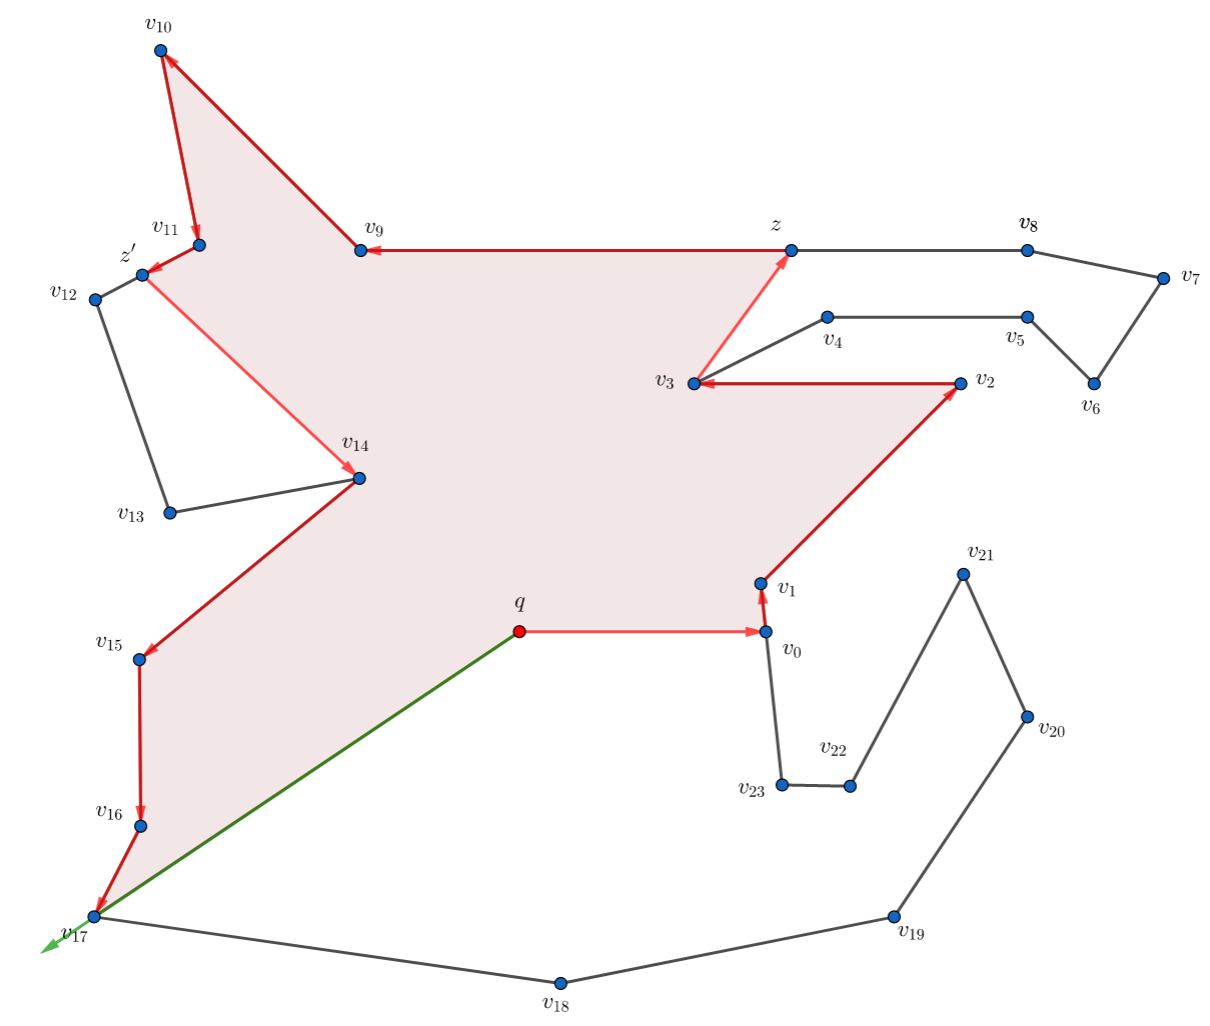
\includegraphics[width=0.70 \paperwidth]{images/Ejecucion/e22.png}
\end{frame}

\begin{frame}
  \centering 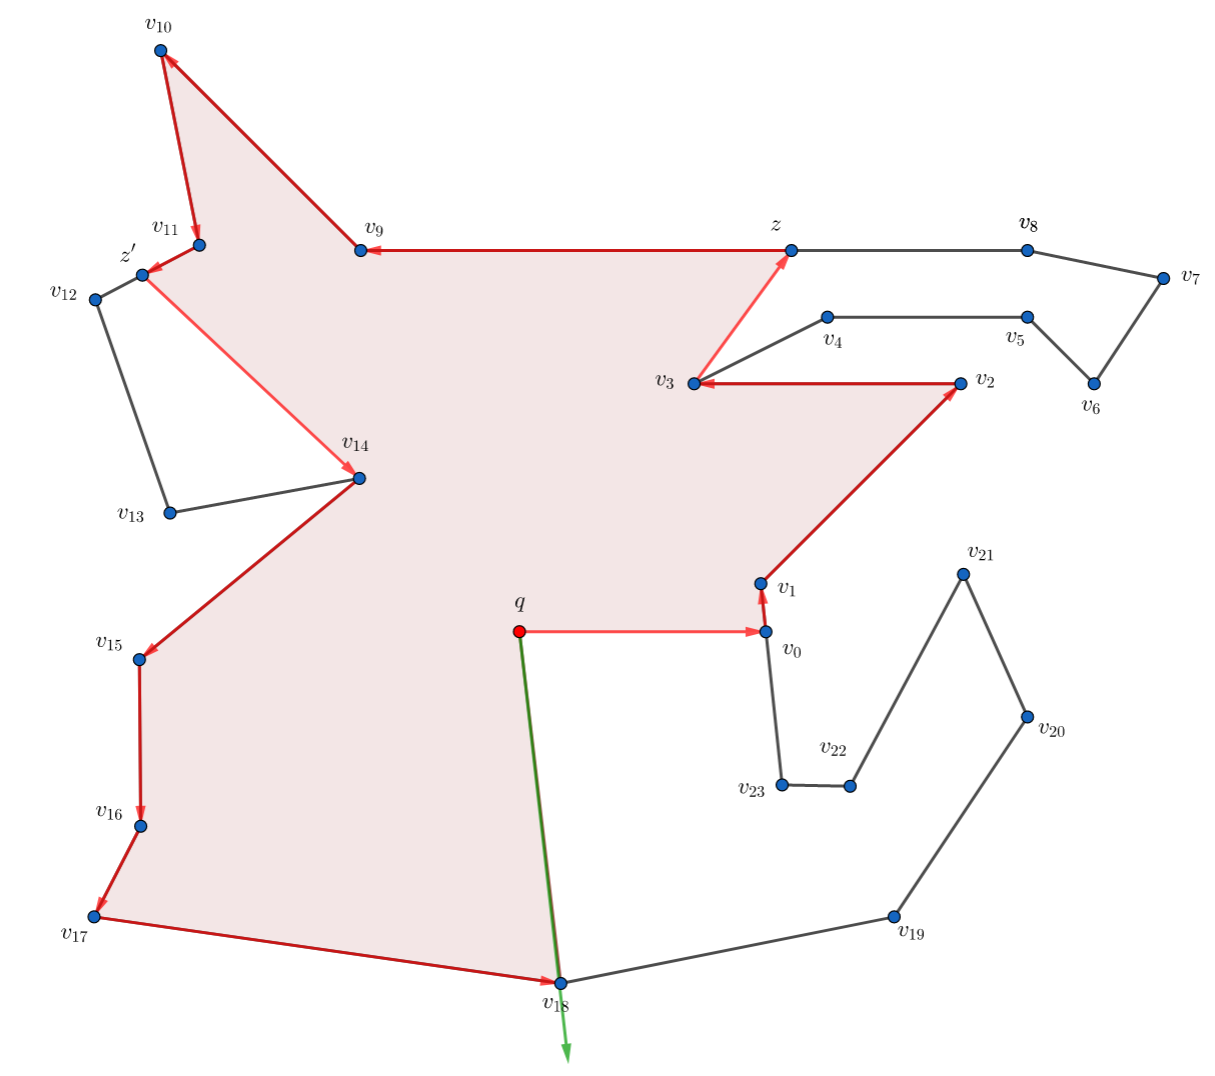
\includegraphics[width=0.70 \paperwidth]{images/Ejecucion/e23.png}
\end{frame}

\begin{frame}
  \centering 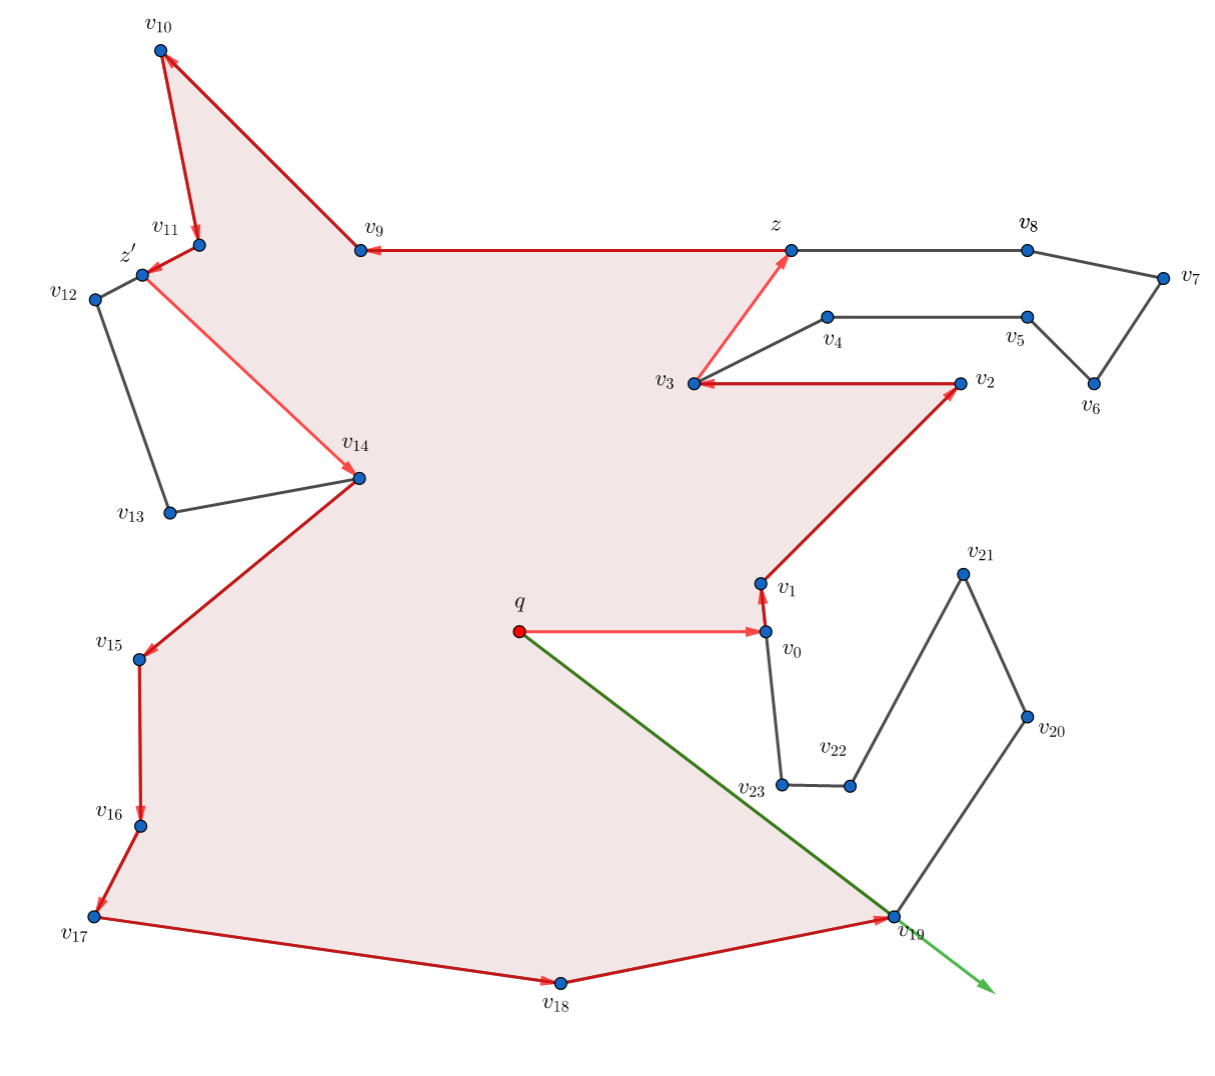
\includegraphics[width=0.70 \paperwidth]{images/Ejecucion/e24.png}
\end{frame}

\begin{frame}
  \centering 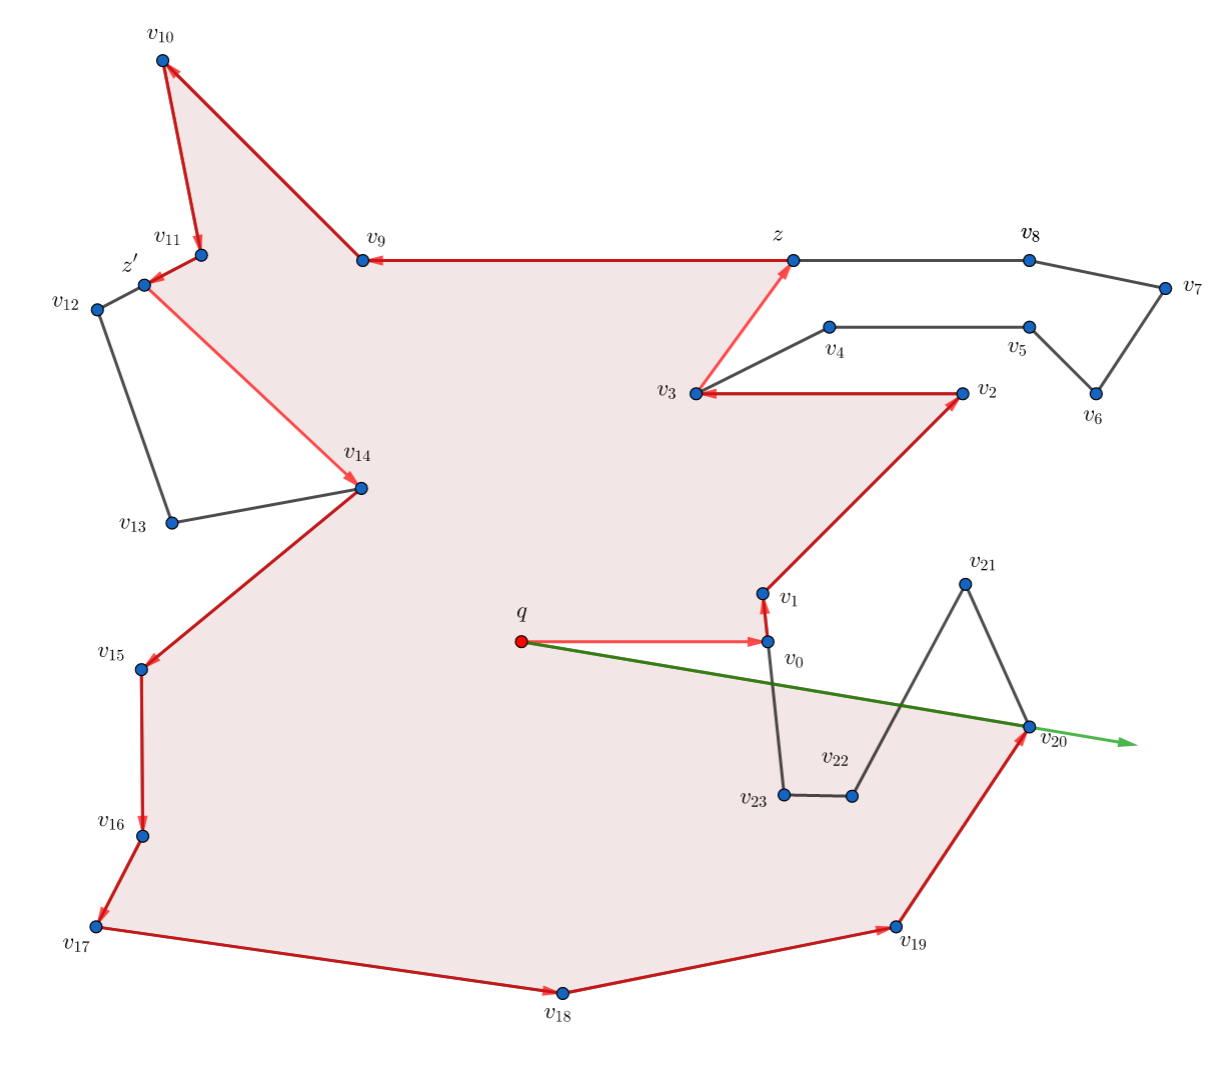
\includegraphics[width=0.70 \paperwidth]{images/Ejecucion/e25.png}
\end{frame}

\begin{frame}
  \centering 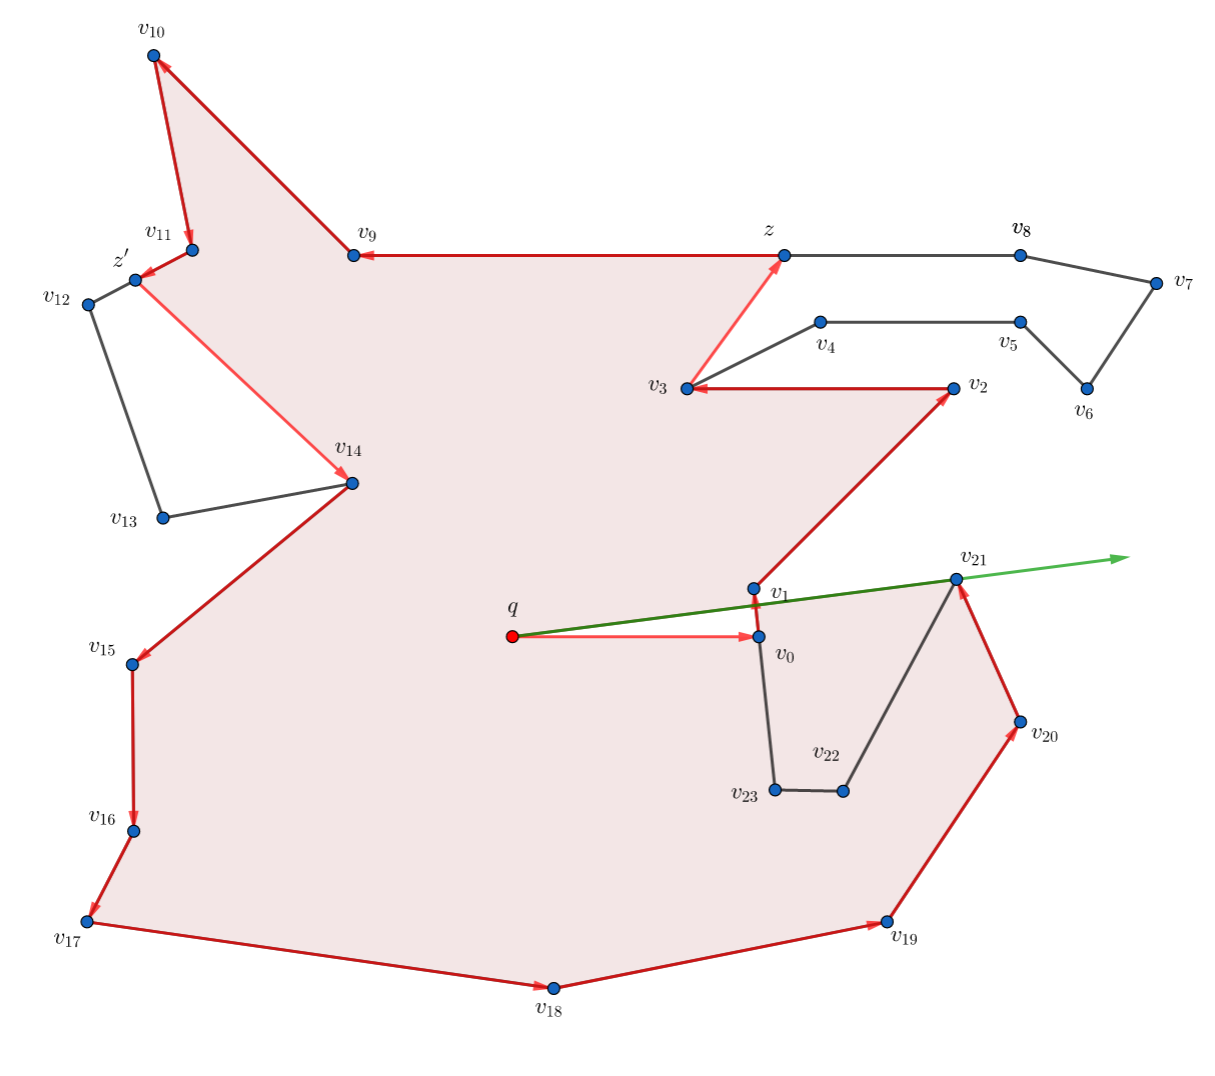
\includegraphics[width=0.70 \paperwidth]{images/Ejecucion/e26.png}
\end{frame}

\begin{frame}
  \centering 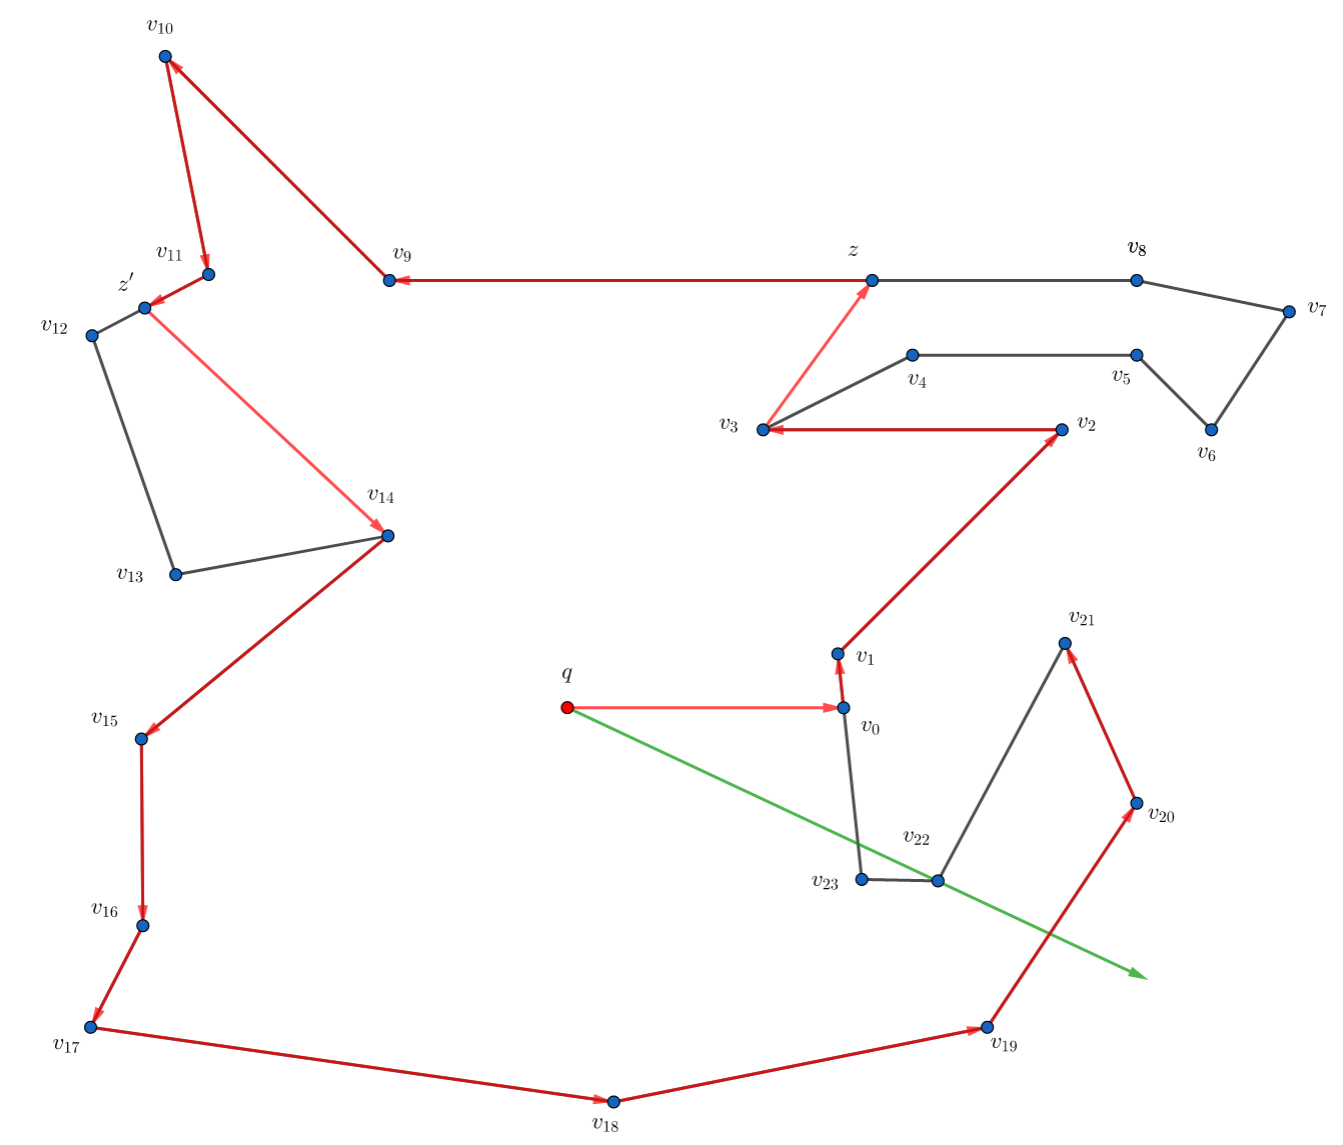
\includegraphics[width=0.70 \paperwidth]{images/Ejecucion/e27.png}
\end{frame}

\begin{frame}
  \centering 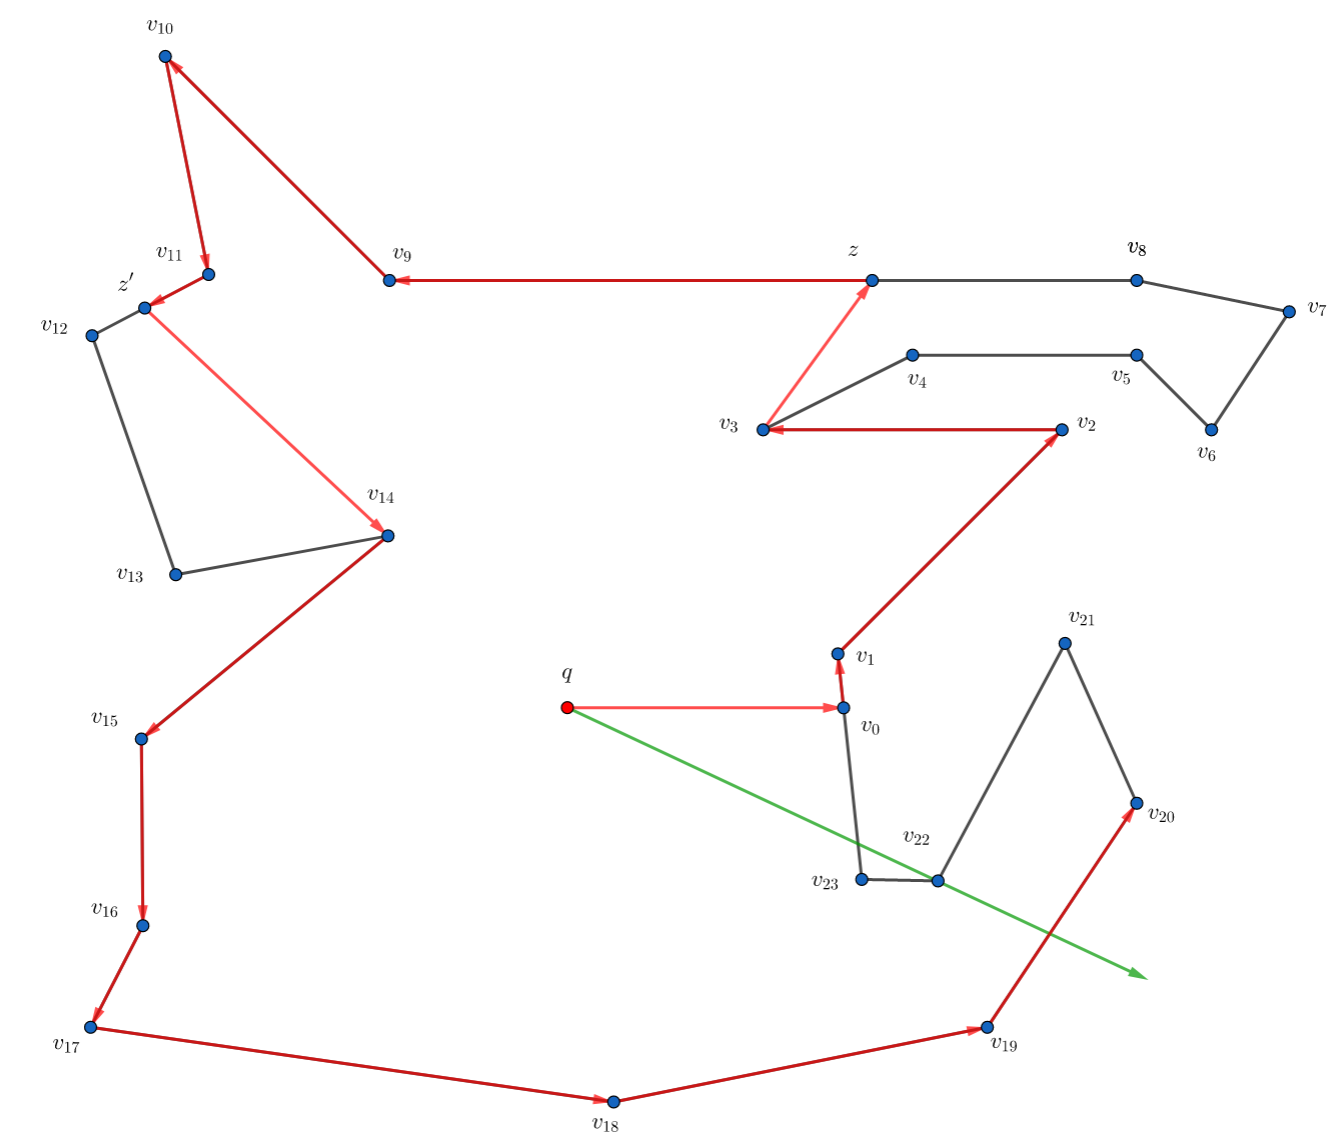
\includegraphics[width=0.70 \paperwidth]{images/Ejecucion/e28.png}
\end{frame}

\begin{frame}
  \centering 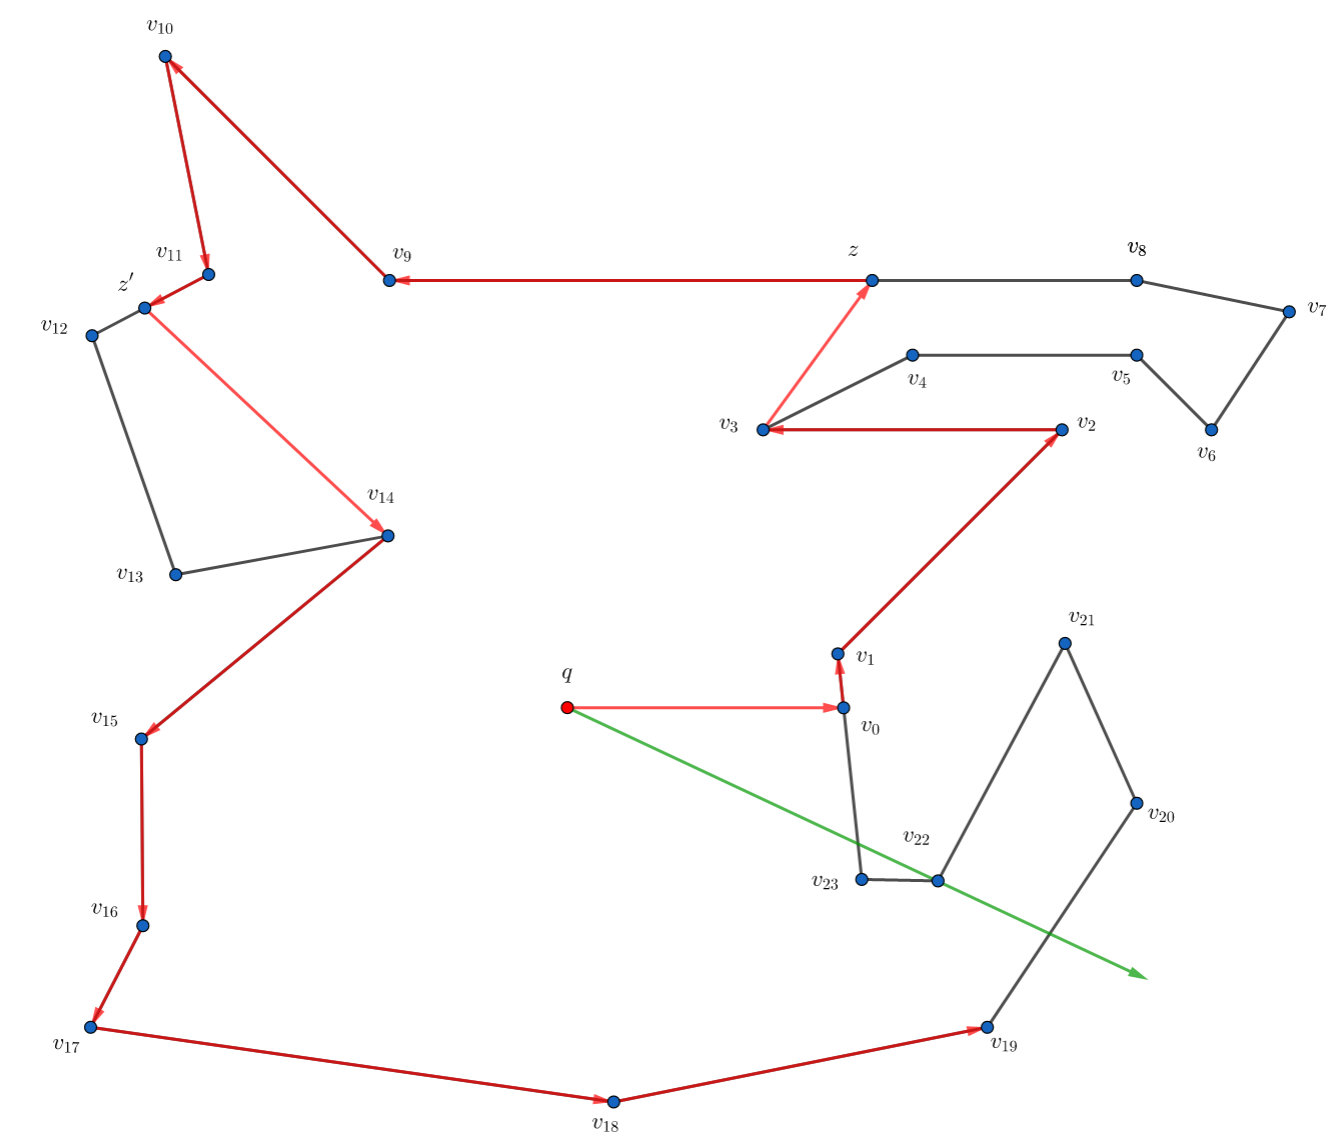
\includegraphics[width=0.70 \paperwidth]{images/Ejecucion/e29.png}
\end{frame}

\begin{frame}
  \centering 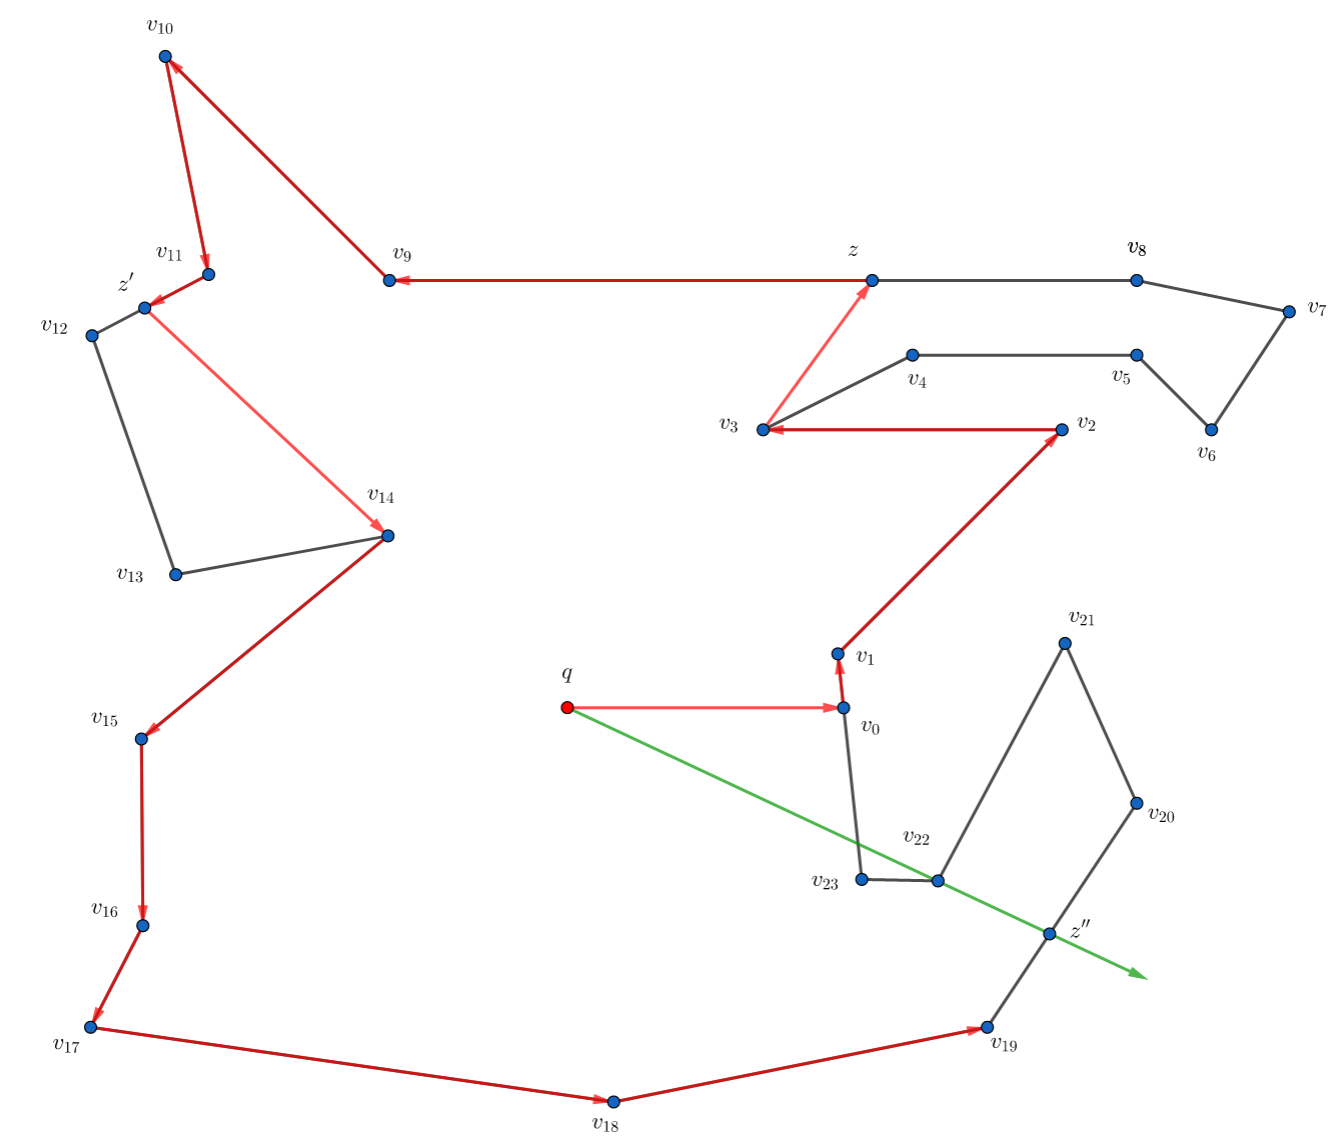
\includegraphics[width=0.70 \paperwidth]{images/Ejecucion/e30.png}
\end{frame}

\begin{frame}
  \centering 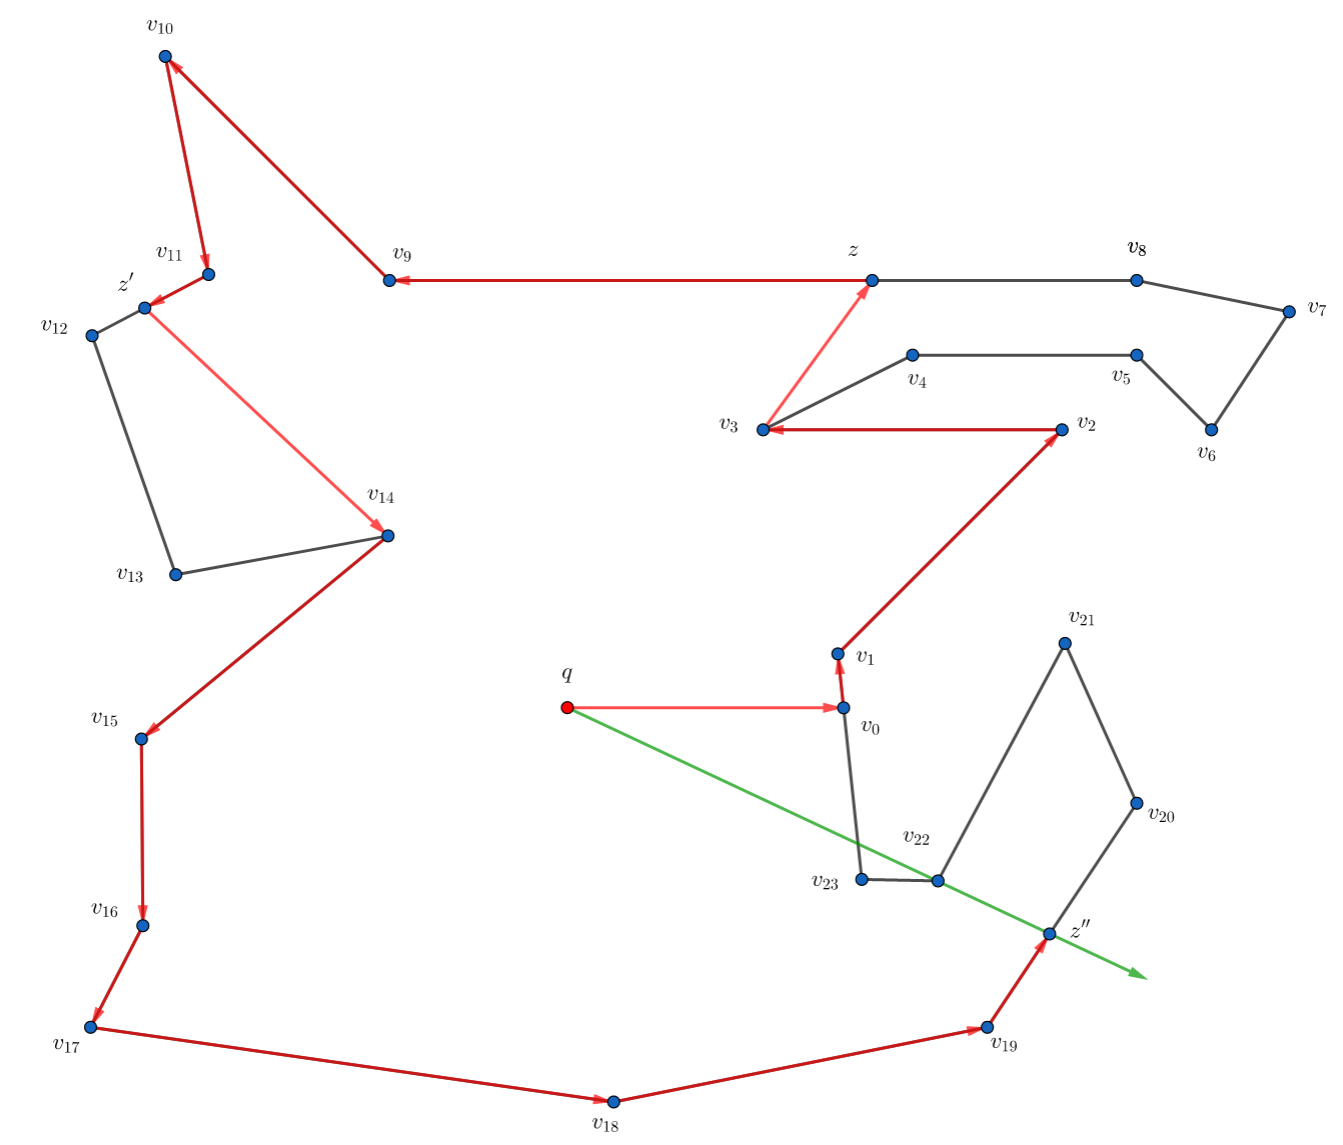
\includegraphics[width=0.70 \paperwidth]{images/Ejecucion/e31.png}
\end{frame}

\begin{frame}
  \centering 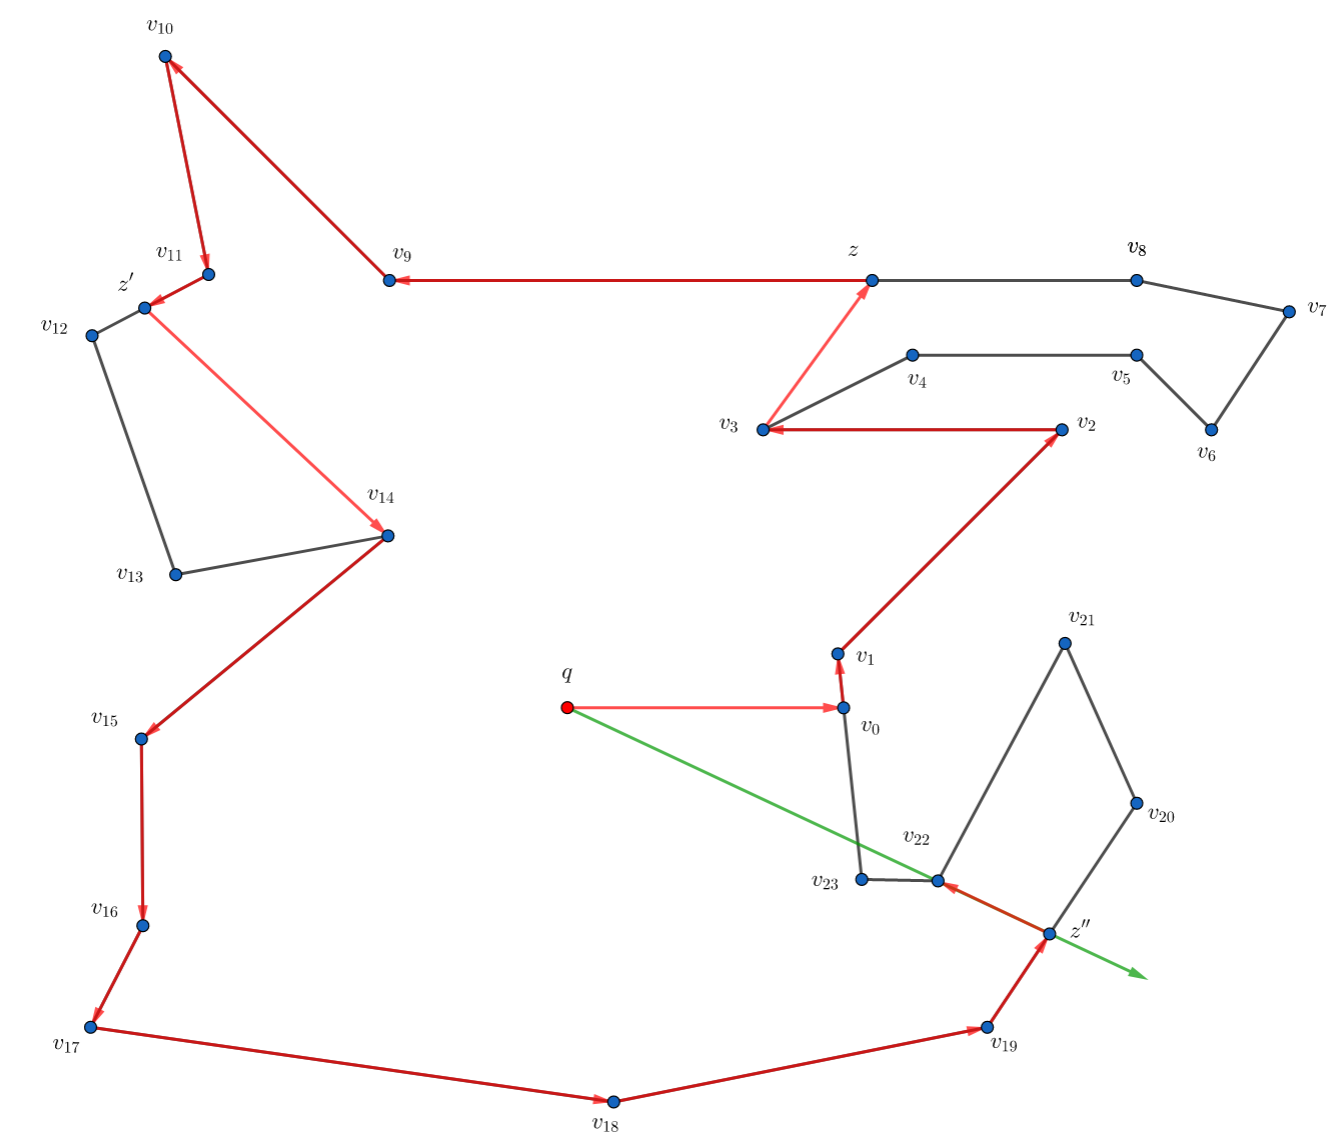
\includegraphics[width=0.70 \paperwidth]{images/Ejecucion/e32.png}
\end{frame}

\begin{frame}
  \centering 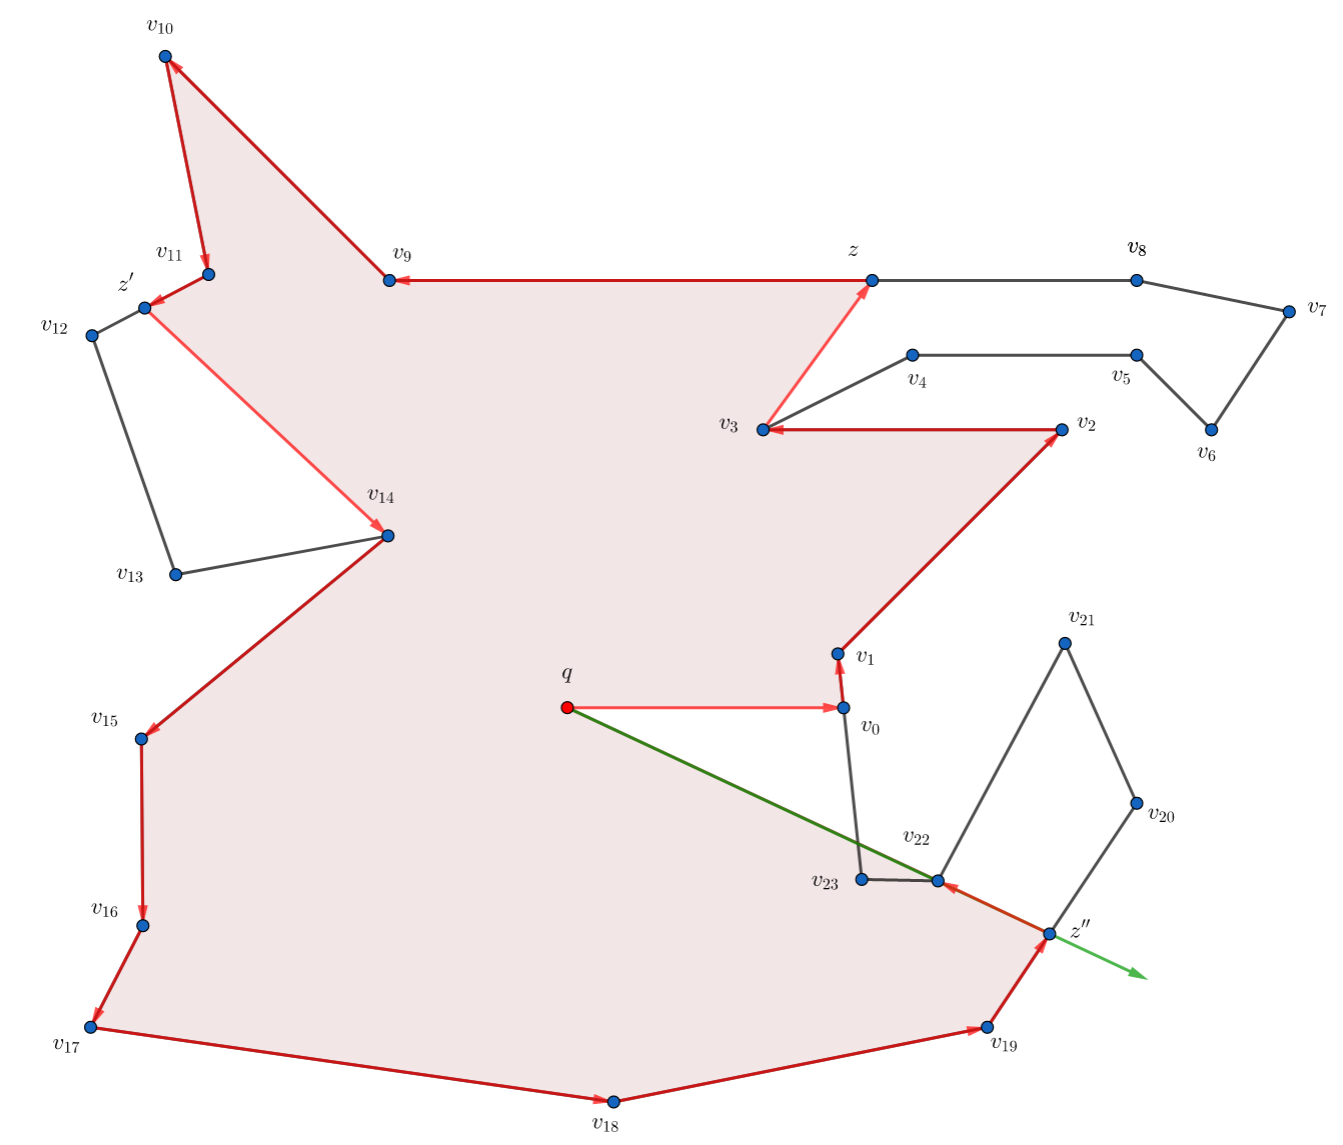
\includegraphics[width=0.70 \paperwidth]{images/Ejecucion/e33.png}
\end{frame}

\begin{frame}
  \centering 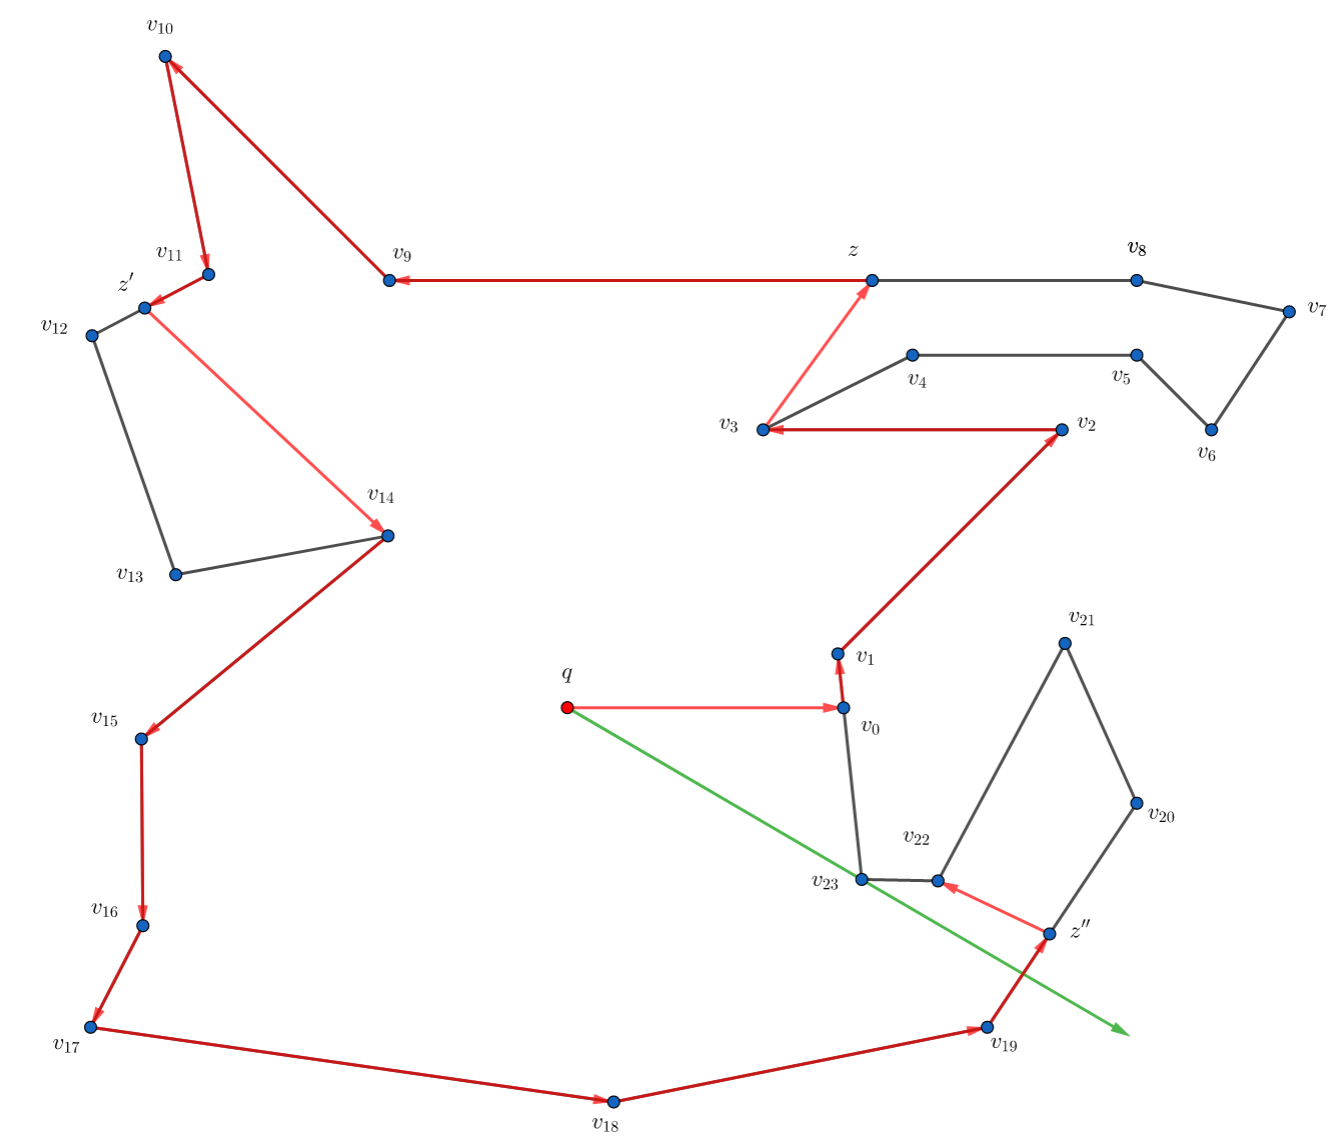
\includegraphics[width=0.70 \paperwidth]{images/Ejecucion/e34.png}
\end{frame}

\begin{frame}
  \centering 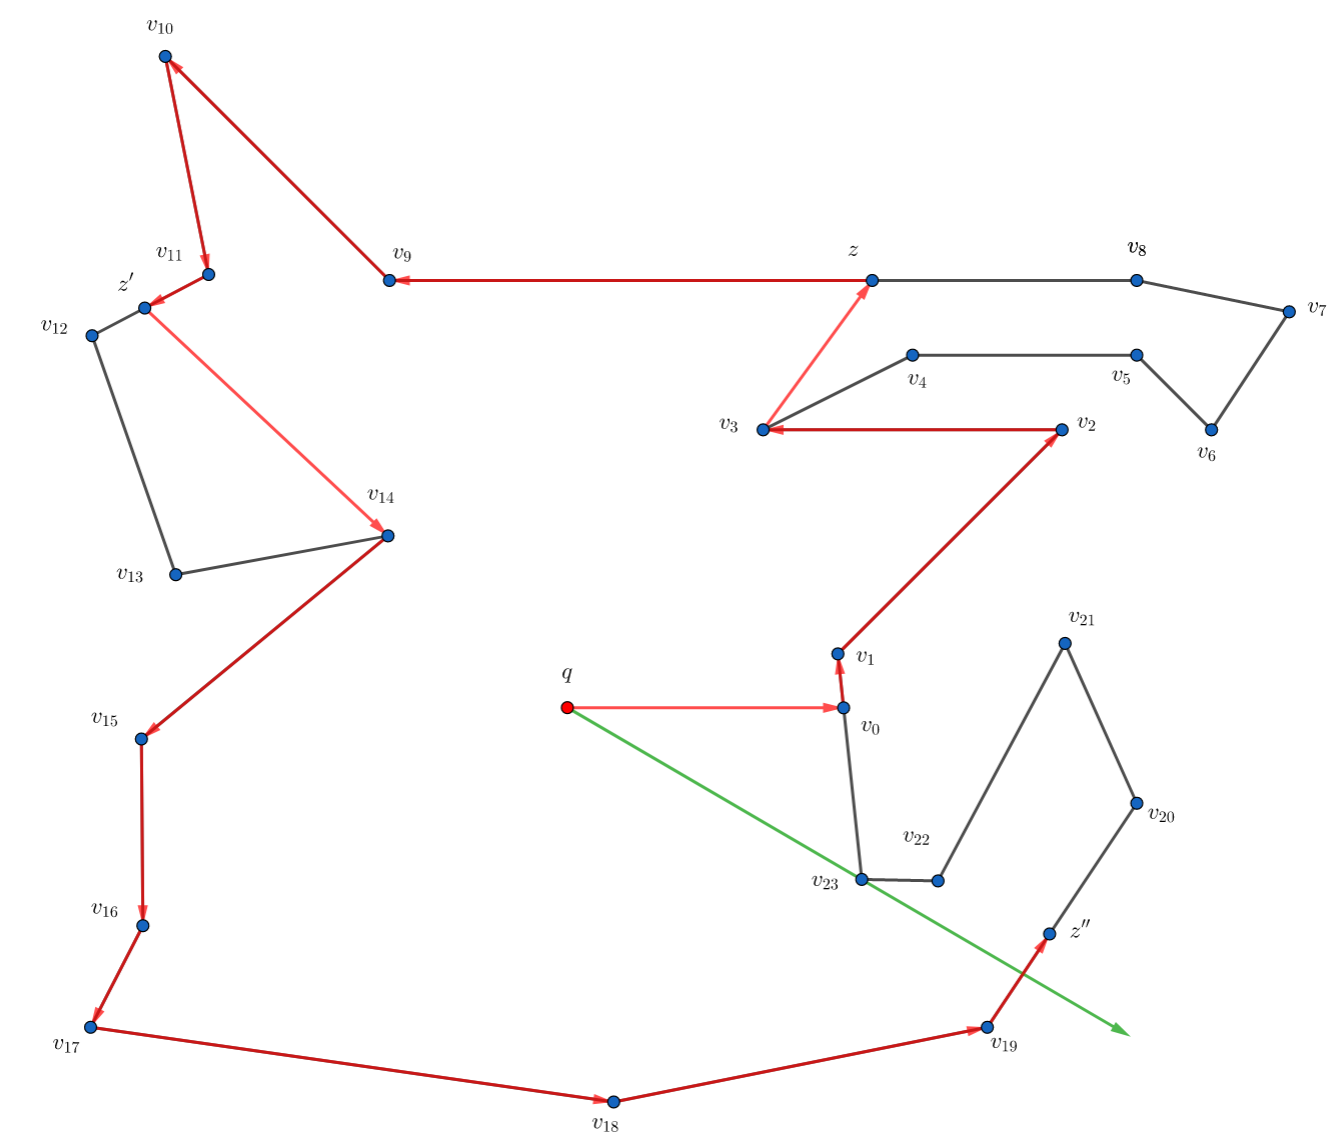
\includegraphics[width=0.70 \paperwidth]{images/Ejecucion/e35.png}
\end{frame}

\begin{frame}
  \centering 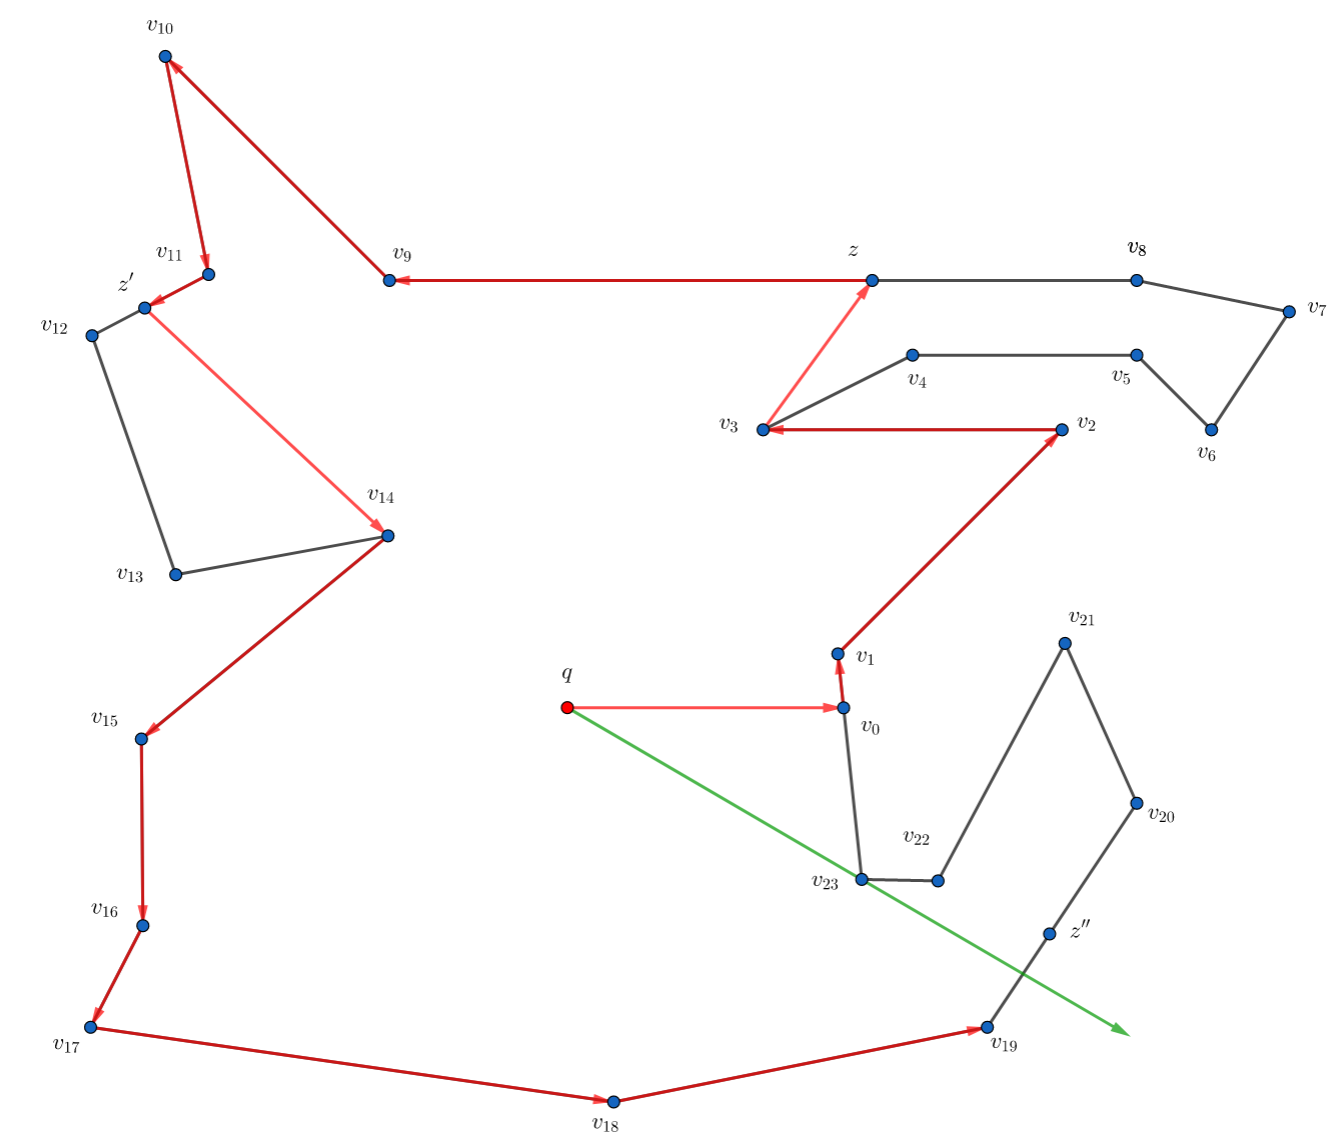
\includegraphics[width=0.70 \paperwidth]{images/Ejecucion/e36.png}
\end{frame}

\begin{frame}
  \centering 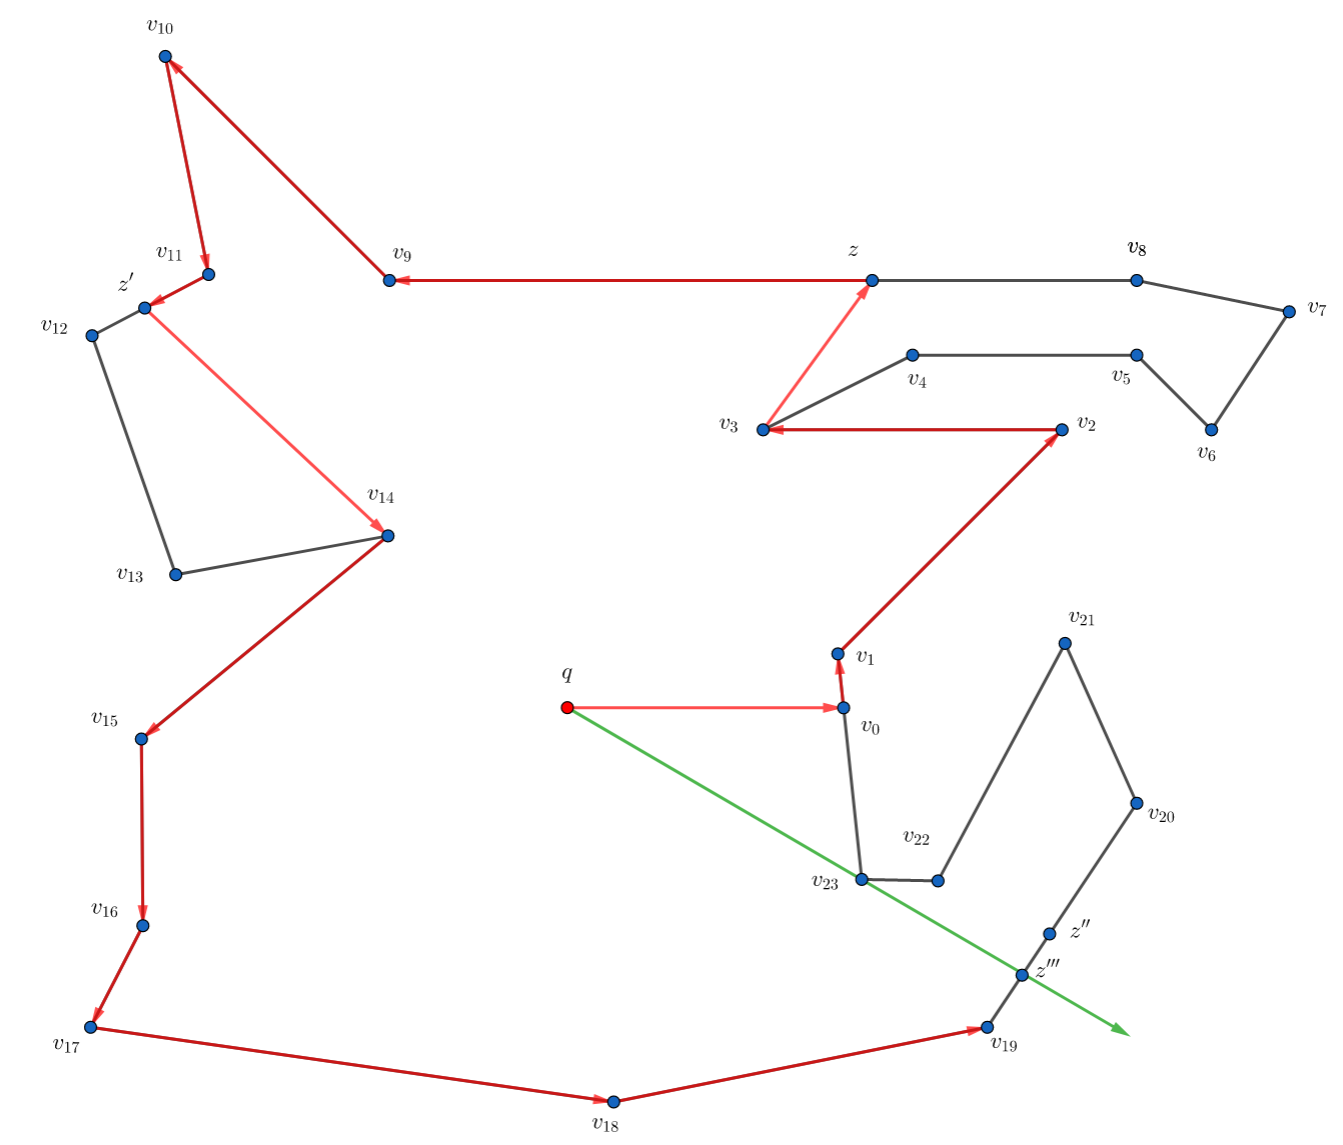
\includegraphics[width=0.70 \paperwidth]{images/Ejecucion/e37.png}
\end{frame}

\begin{frame}
  \centering 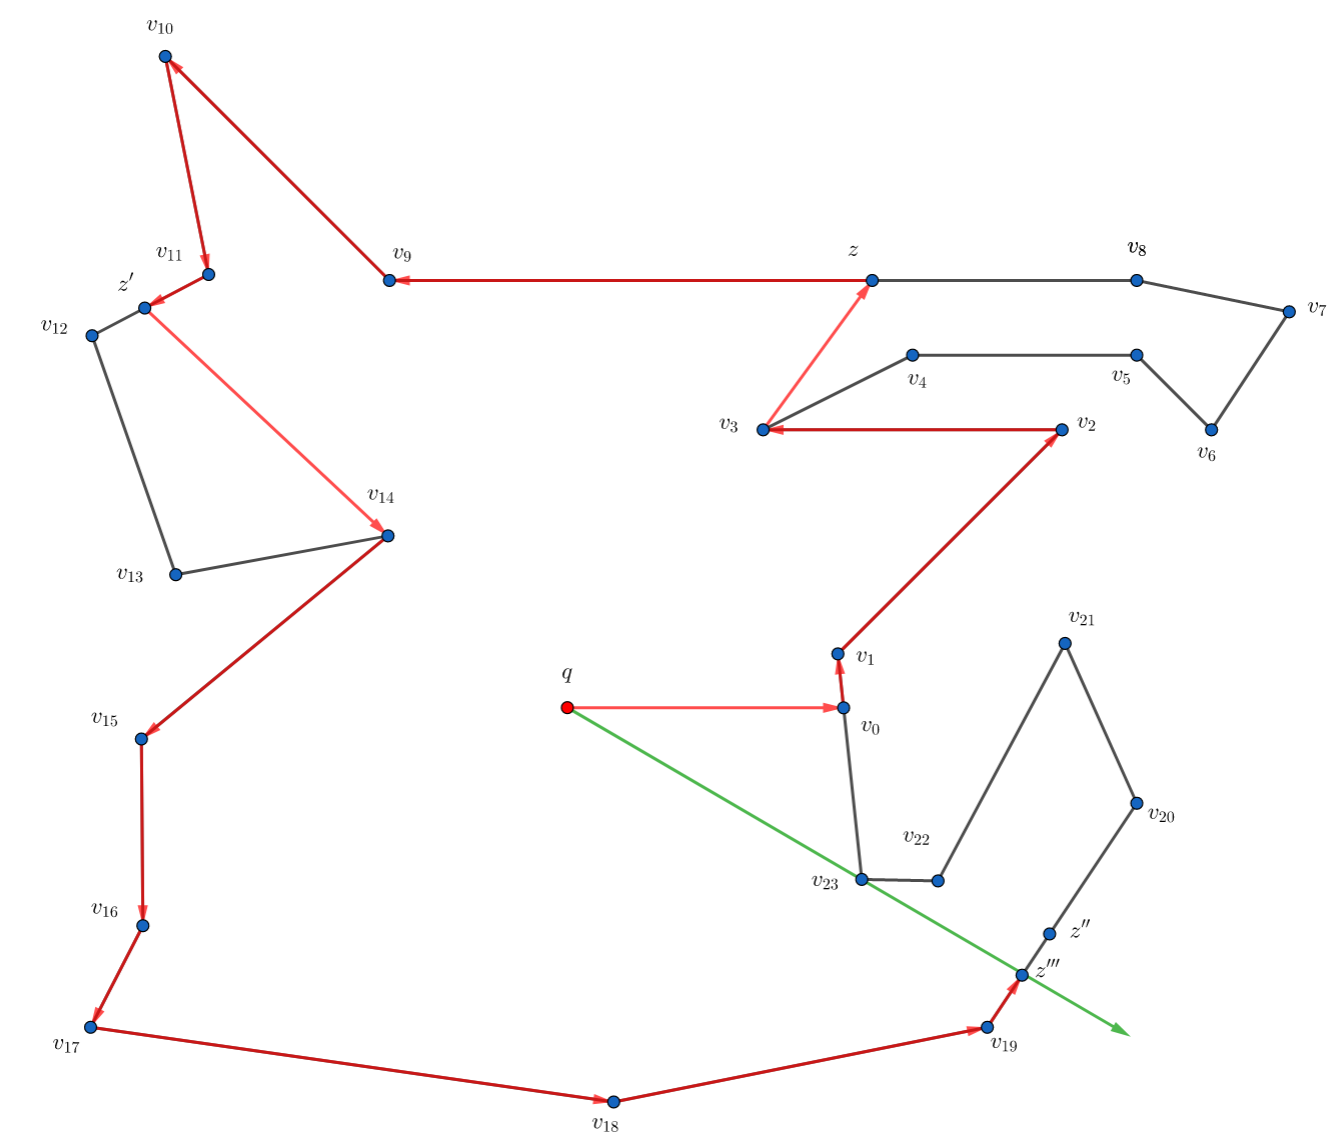
\includegraphics[width=0.70 \paperwidth]{images/Ejecucion/e38.png}
\end{frame}

\begin{frame}
  \centering 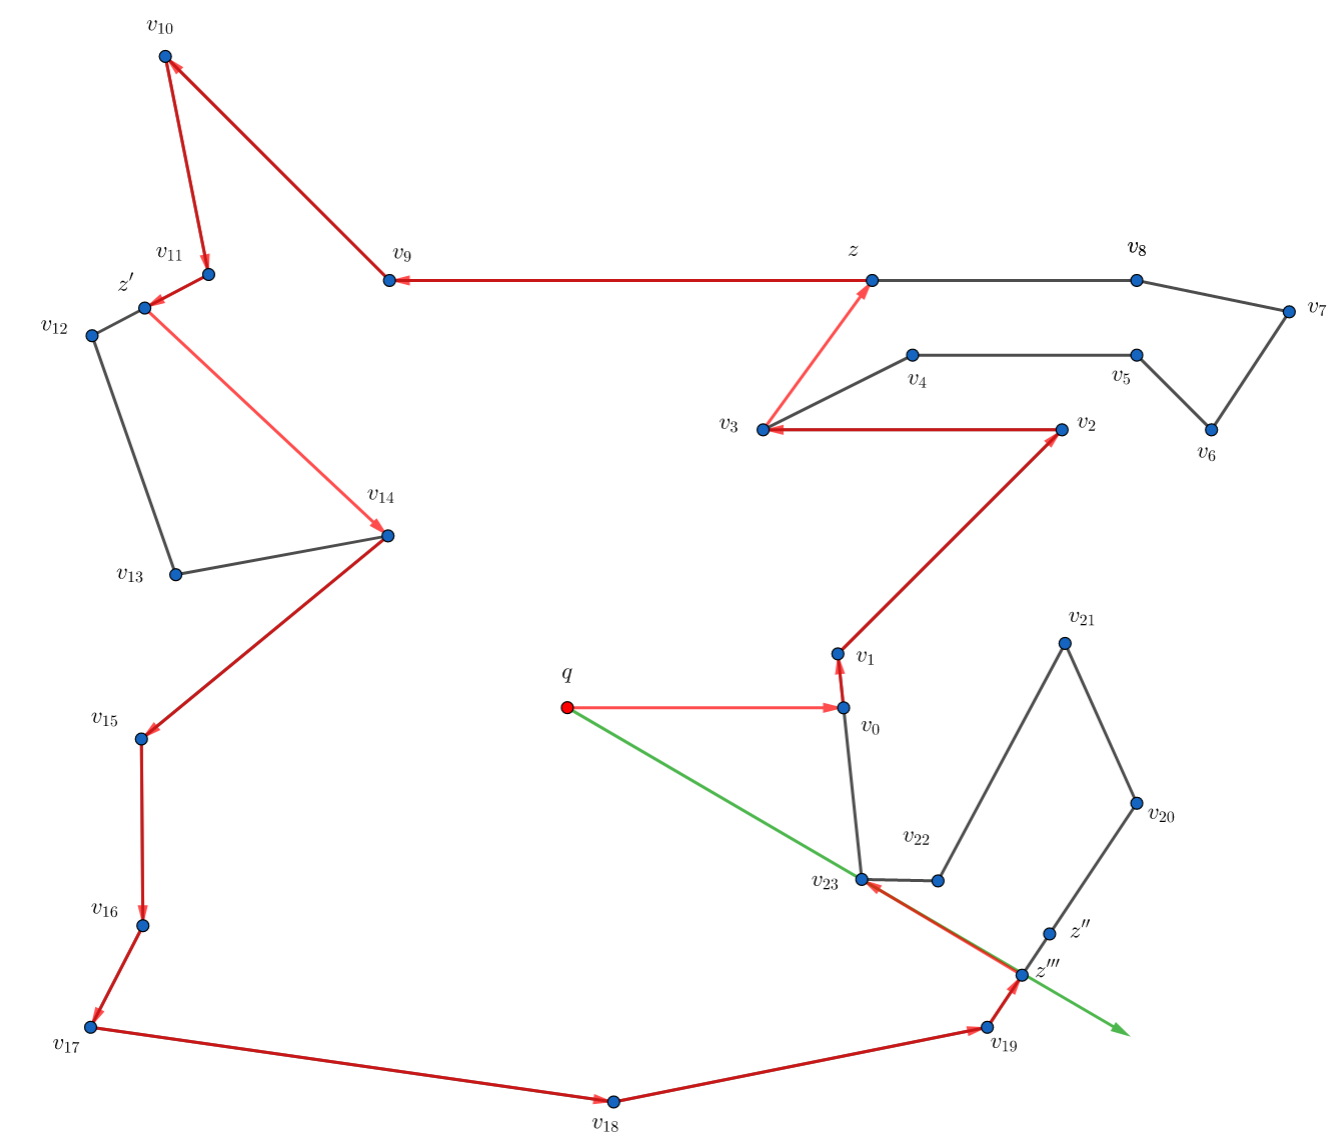
\includegraphics[width=0.70 \paperwidth]{images/Ejecucion/e39.png}
\end{frame}

\begin{frame}
  \centering 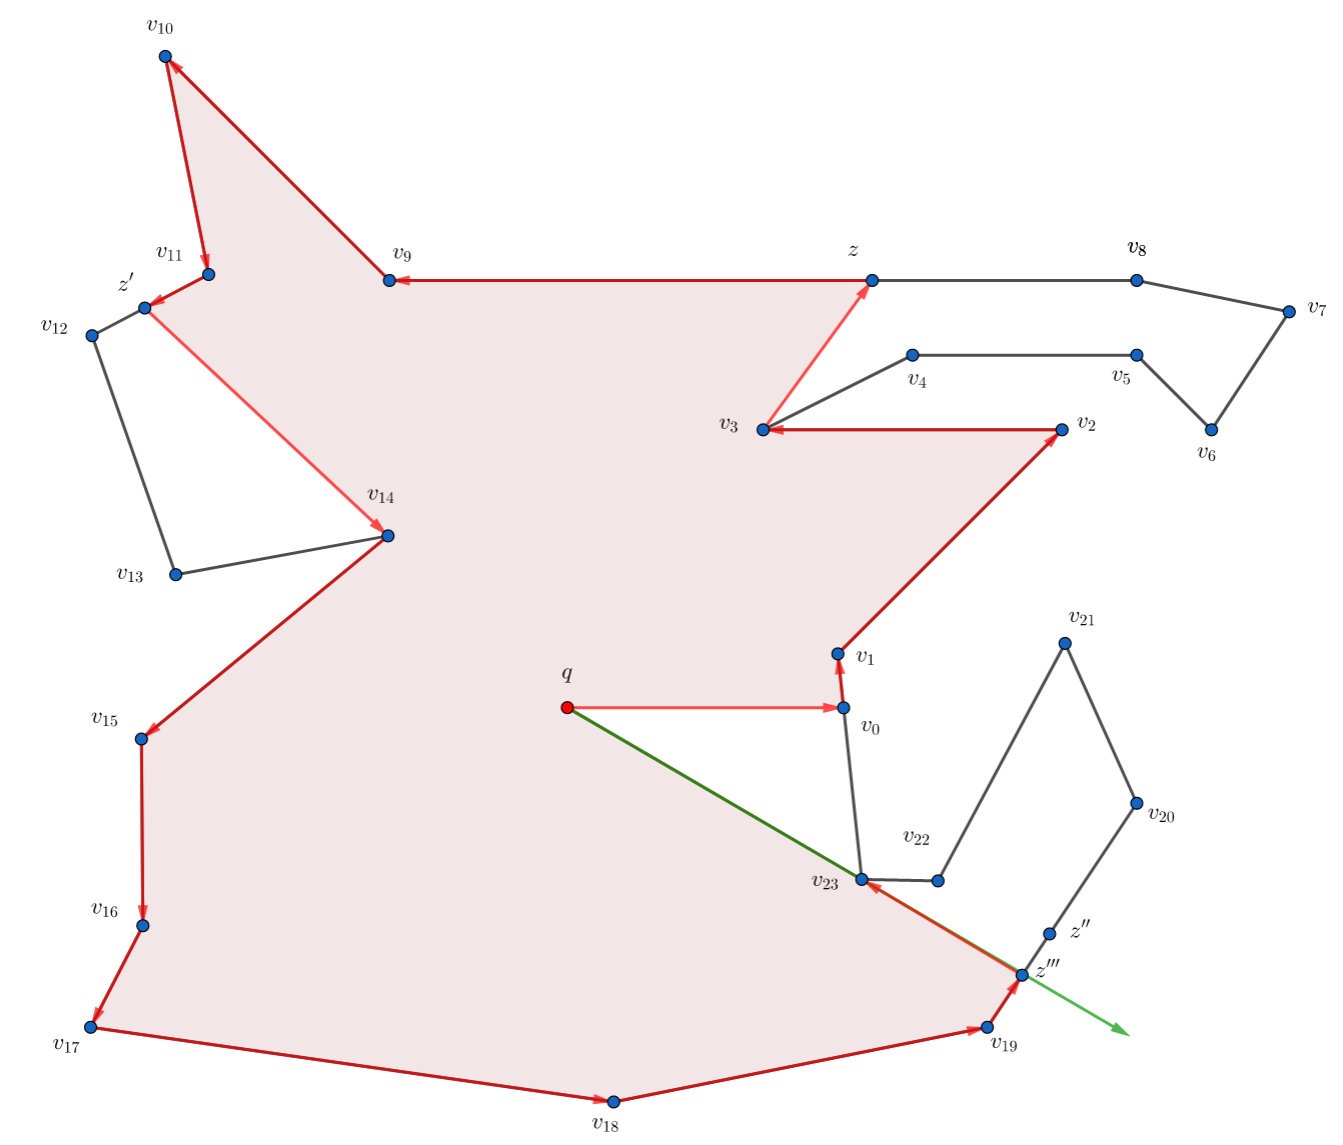
\includegraphics[width=0.70 \paperwidth]{images/Ejecucion/e40.png}
\end{frame}

\begin{frame}
  \centering 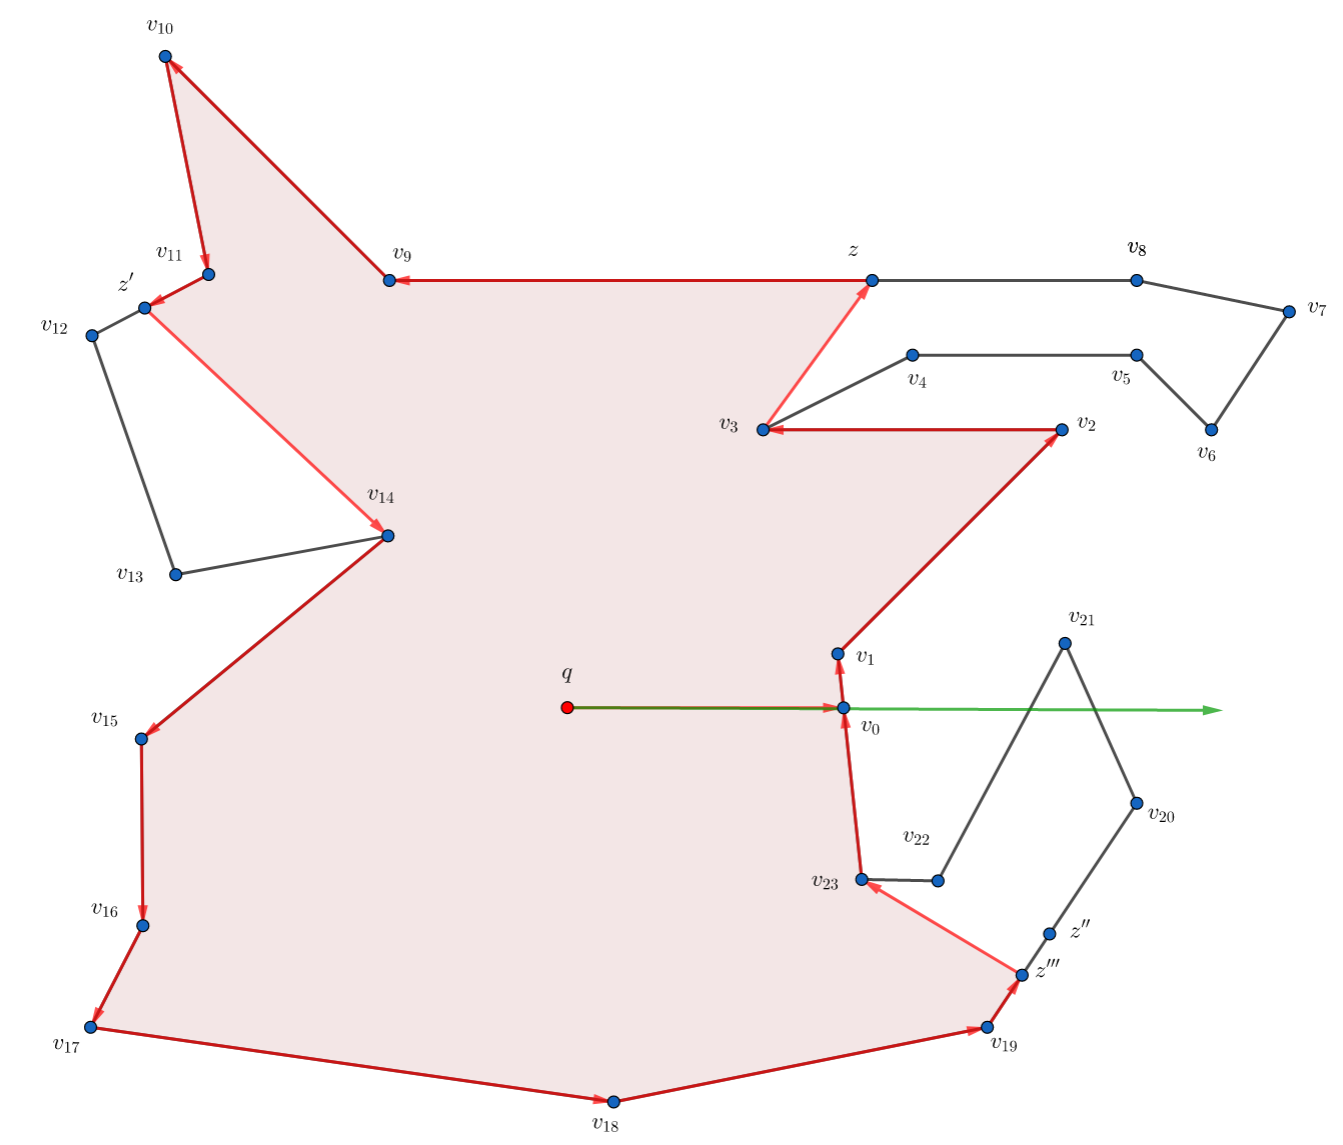
\includegraphics[width=0.70 \paperwidth]{images/Ejecucion/e41.png}
\end{frame}

\begin{frame}
  \centering 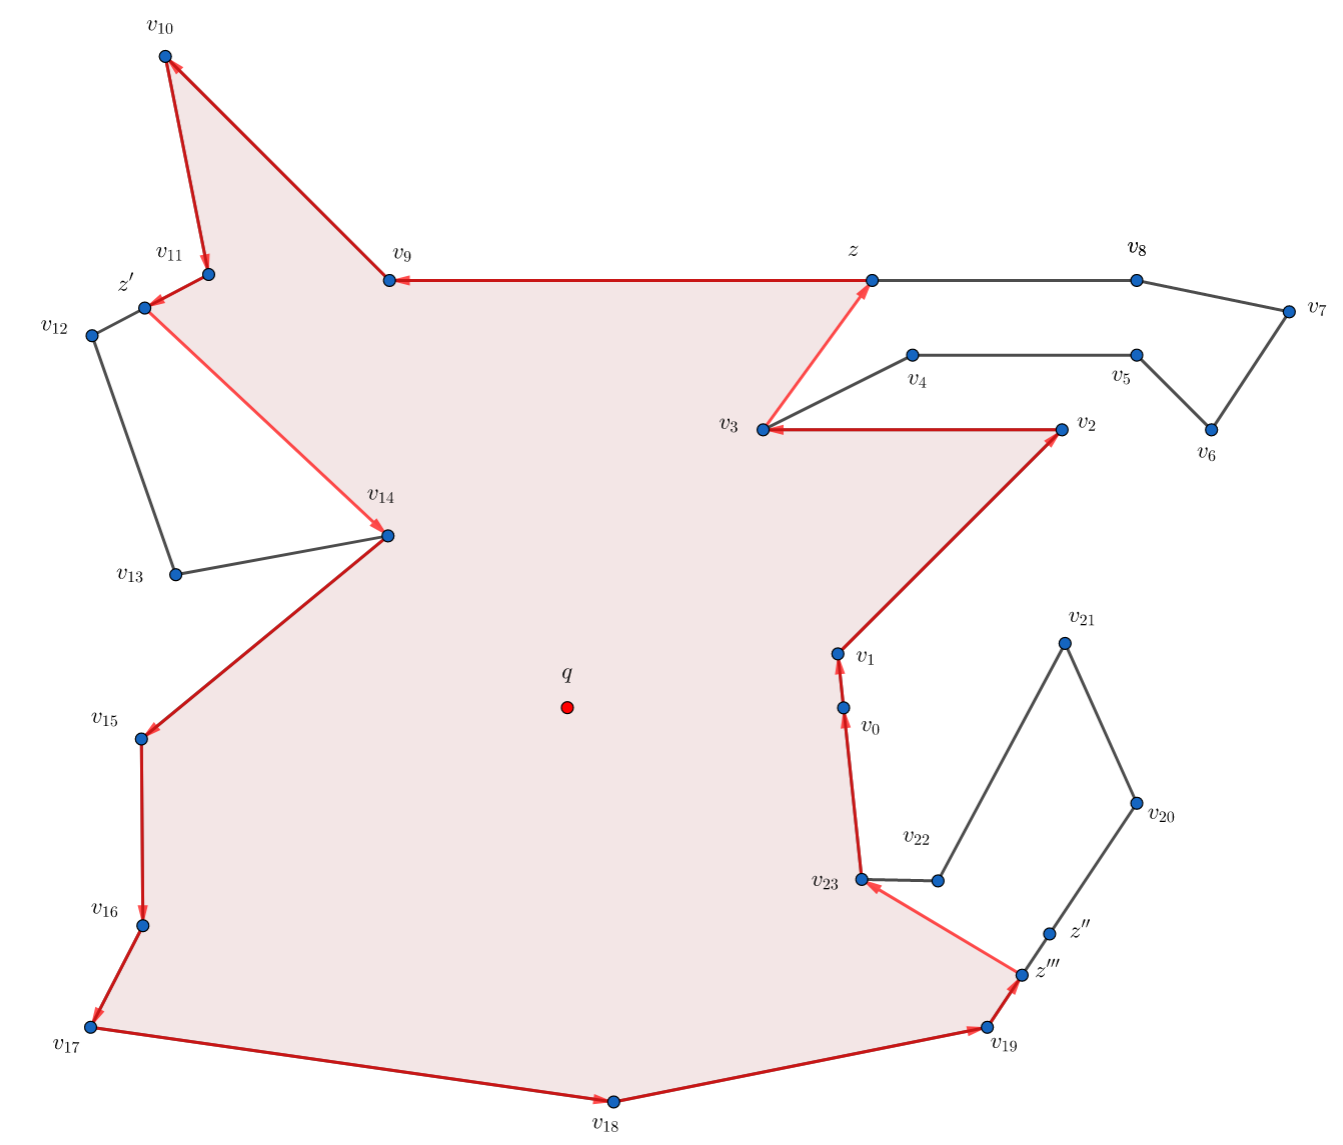
\includegraphics[width=0.70 \paperwidth]{images/Ejecucion/e42.png}
\end{frame}

\subsection{Análisis de complejidad.}

\begin{frame}
  \frametitle{Análisis de complejidad.}
  \begin{enumerate}
  \item Encontrar el punto de intersección del primer rayo a partir de $q$ con la
    frontera del polígono simple $P$, lo realizamos en $\mathcal{O}(\log n)$ con una
    búsqueda en el orden del polígono.
  \item En cada paso de la iteración guardamos cada vértice una vez en una pila. Recorrer nuestro
    polígono nos toma $\mathcal{O}(n)$.
  \item Encontrar la intersección del rayo con la arista incidente nos toma $\mathcal{O}(1)$, pues
    es suficiente hacer pop en la pila usada.
  \item Verificar en cada iteración la dirección del vértice siguiente lo podemos realizar en $\mathcal{O}(1)$.
  \end{enumerate}
\end{frame}

\subsection{Casos especiales.}

\begin{frame}
  \frametitle{Casos especiales.}
  Existen dos casos espciales para encontrar $V(q)$ de $P$, estos son
  \begin{itemize}
  \item $q$ está fuera de $P$ y se encuentra dentro de la envolvente convexa del polígono simple $P$.
  \item $q$ está fuera de $P$ y se encuentra fuera de la envolvente convexa del polígono simple $P$.
  \end{itemize}
\end{frame}

\begin{frame}
  \frametitle{Caso 1.}
  \centering 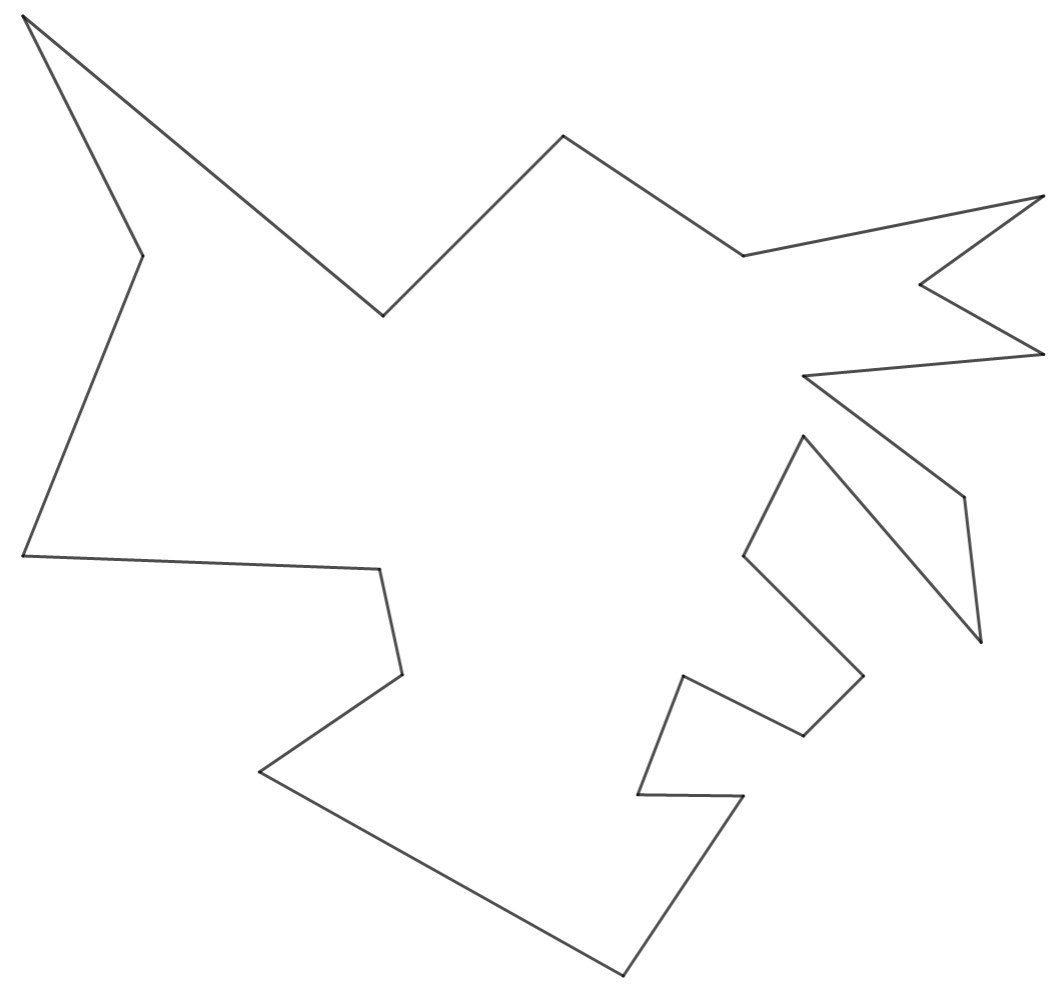
\includegraphics[width=0.50 \paperwidth]{images/CasosQExterno/P.png}
\end{frame}

\begin{frame}
  \frametitle{Caso 1.}
  \centering 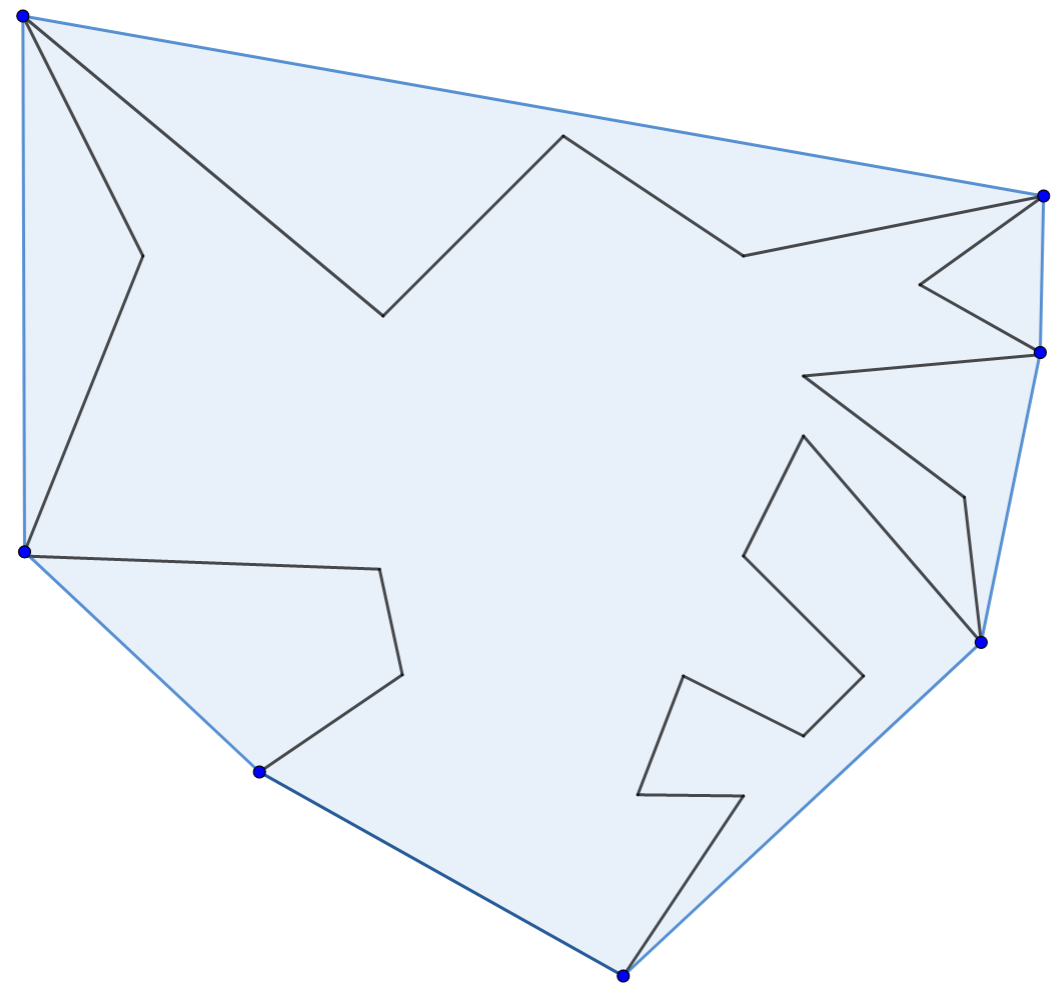
\includegraphics[width=0.50 \paperwidth]{images/CasosQExterno/P01.png}
\end{frame}

\begin{frame}
  \frametitle{Caso 1.}
  \centering 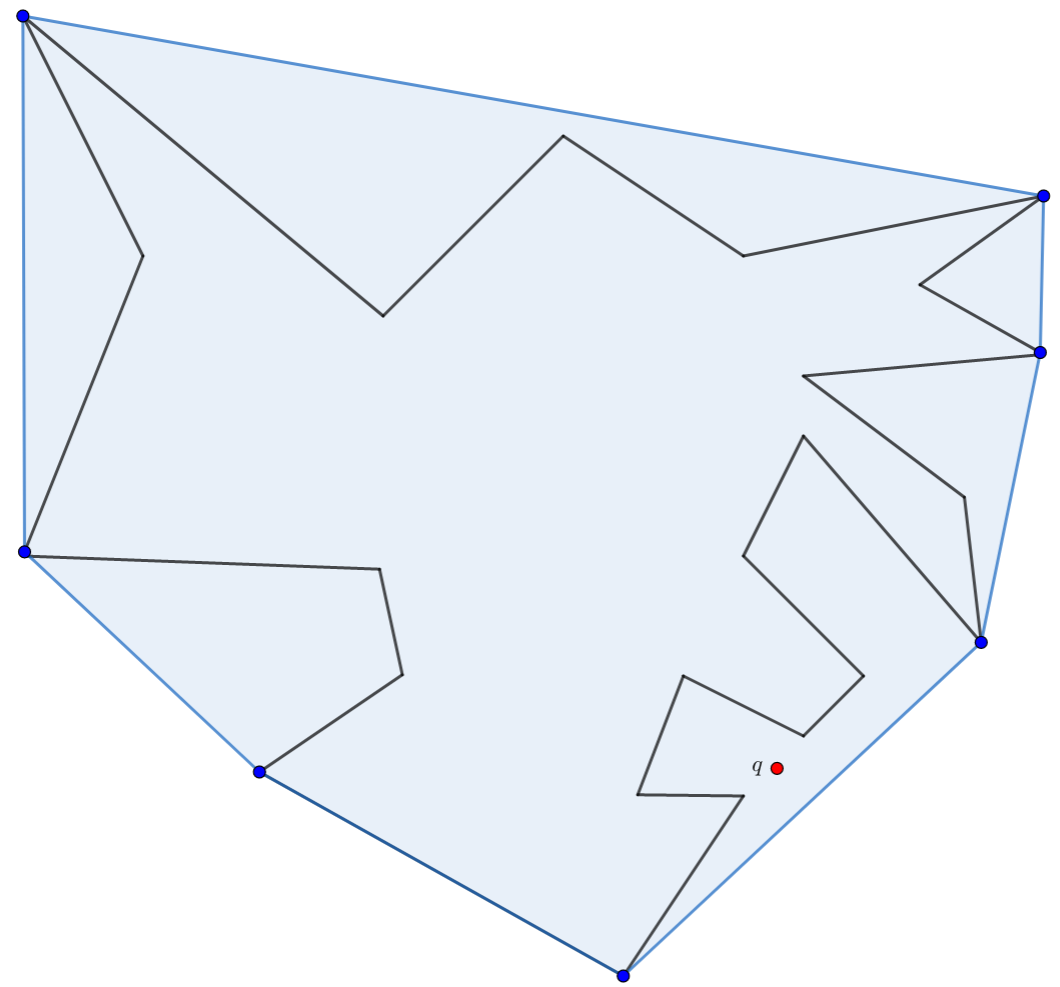
\includegraphics[width=0.50 \paperwidth]{images/CasosQExterno/P02.png}
\end{frame}

\begin{frame}
  \frametitle{Caso 1.}
  \centering 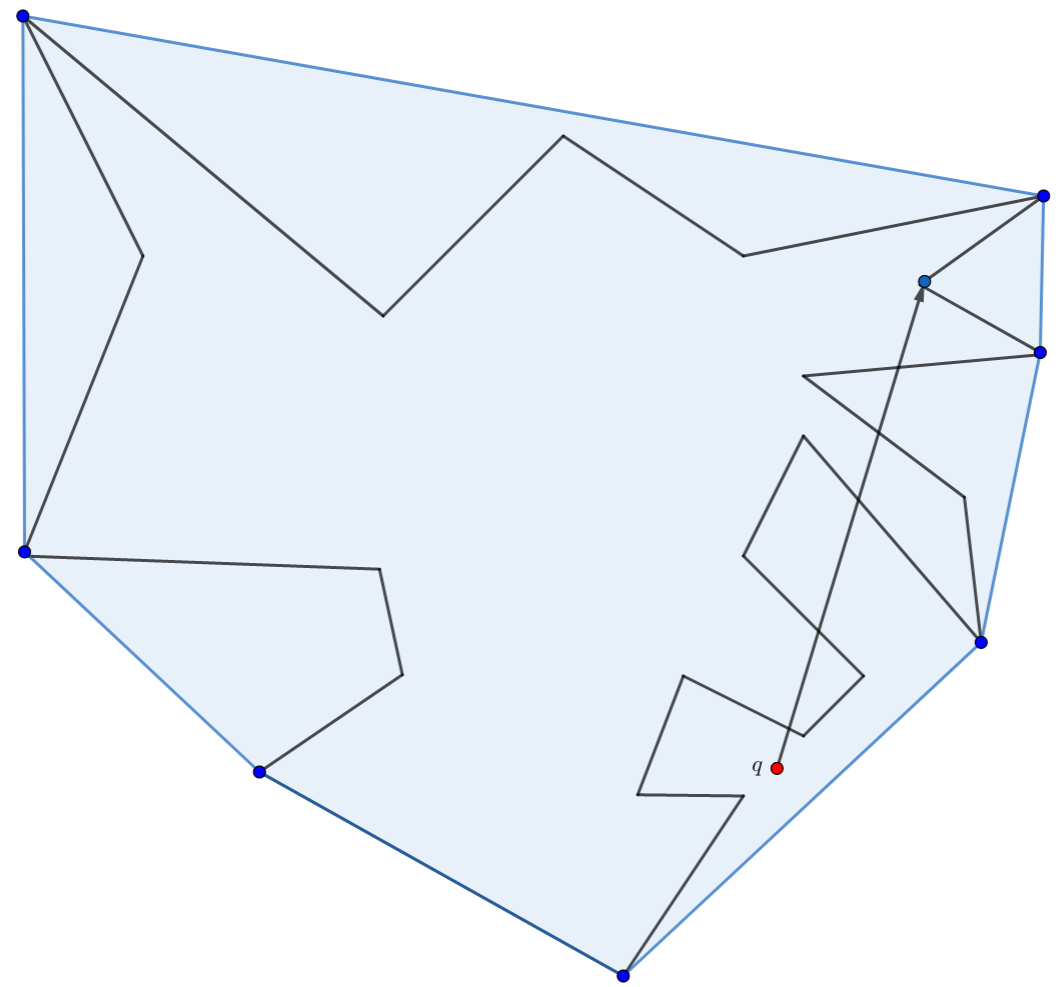
\includegraphics[width=0.50 \paperwidth]{images/CasosQExterno/P03.png}
\end{frame}

\begin{frame}
  \frametitle{Caso 1.}
  \centering 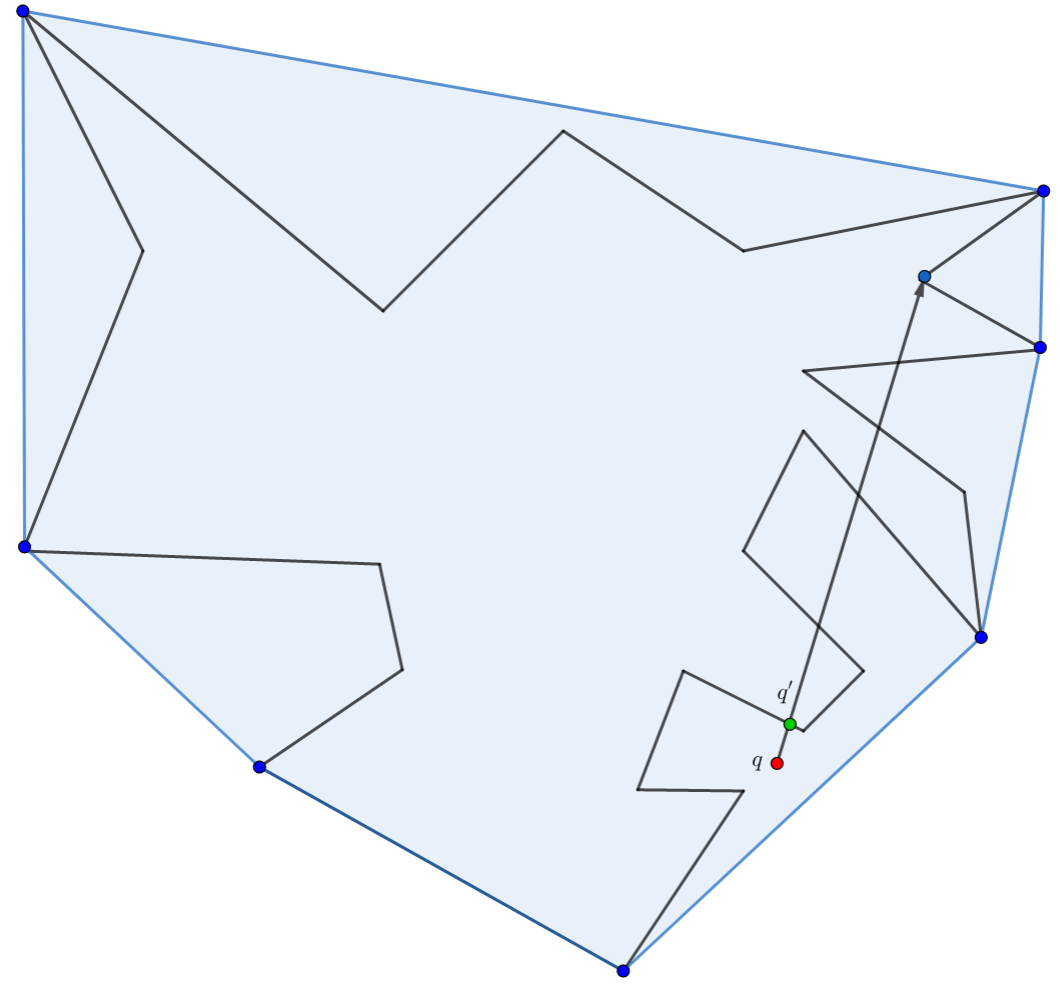
\includegraphics[width=0.50 \paperwidth]{images/CasosQExterno/P04.png}
\end{frame}

\begin{frame}
  \frametitle{Caso 1.}
  \centering 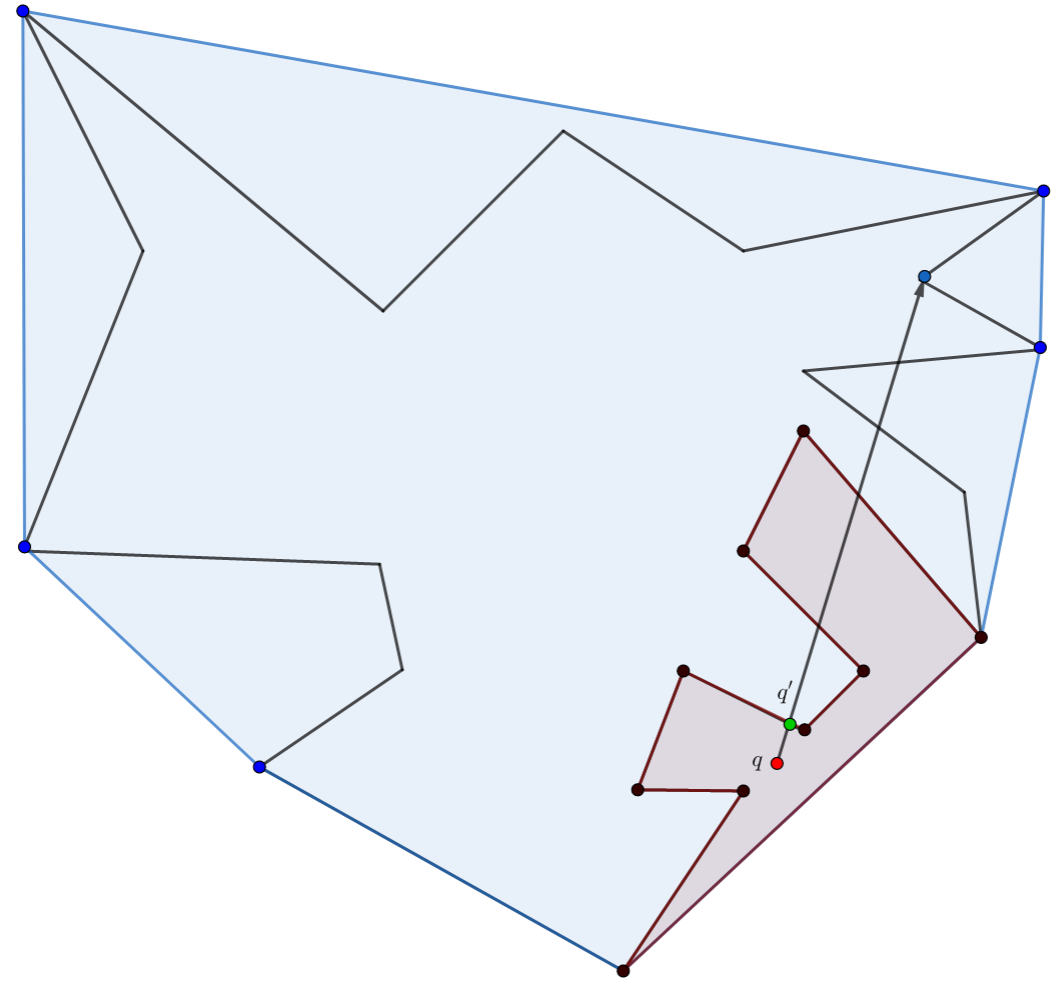
\includegraphics[width=0.50 \paperwidth]{images/CasosQExterno/P05.png}
\end{frame}

\begin{frame}
  \frametitle{Caso 2.}
  \centering 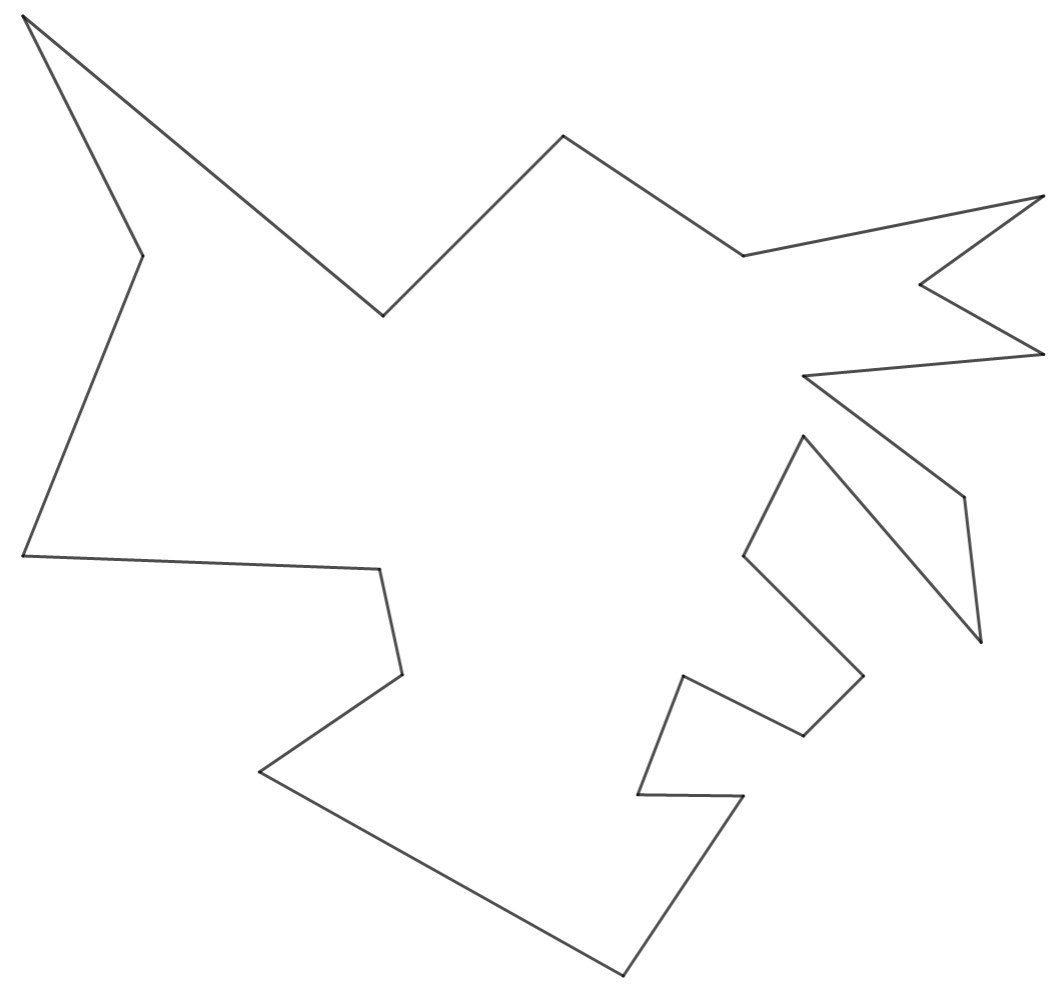
\includegraphics[width=0.50 \paperwidth]{images/CasosQExterno/P.png}
\end{frame}

\begin{frame}
  \frametitle{Caso 2.}
  \centering 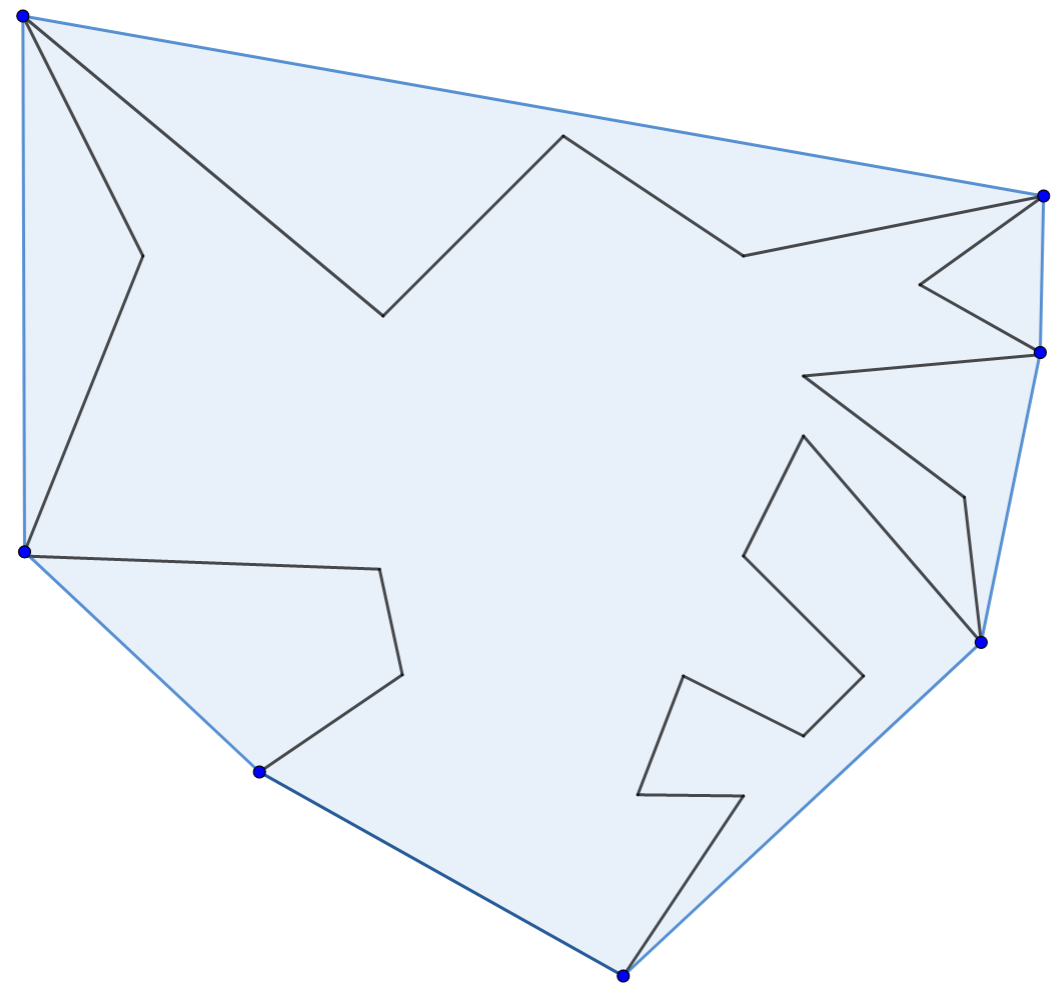
\includegraphics[width=0.50 \paperwidth]{images/CasosQExterno/P01.png}
\end{frame}

\begin{frame}
  \frametitle{Caso 2.}
  \centering \includegraphics[width=0.50 \paperwidth]{images/CasosQExterno/P02F.png}
\end{frame}

\begin{frame}
  \frametitle{Caso 2.}
  \centering \includegraphics[width=0.45 \paperwidth]{images/CasosQExterno/P03F.png}
\end{frame}

\begin{frame}
  \frametitle{Caso 2.}
  \centering \includegraphics[width=0.45 \paperwidth]{images/CasosQExterno/P04F.png}
\end{frame}


\begin{frame}
  \frametitle{Análisis de complejidad.}
  \begin{enumerate}
  \item Encontrar la envolvente convexa de $P$ por medio del algoritmo de Graham-Jao nos toma $\mathcal{O}(n)$.
  \item Encontrar $q'$ o en su defecto las tangentes a $P$ nos toma $\mathcal{O}(\log n)$.
  \item Unir las fronteras encontradas nos toma a lo más $\mathcal{O}(n)$.
  \end{enumerate}
\end{frame}
